\documentclass[11pt]{article}
\usepackage{amssymb}
\usepackage{amsthm}
\usepackage{enumitem}
\usepackage{amsmath, physics}
\usepackage{bm}
\usepackage{adjustbox}
\usepackage{mathrsfs}
\usepackage{graphicx}
\usepackage{siunitx}
\usepackage[mathscr]{euscript}
\usepackage{tikz}
\usepackage{float}

\usetikzlibrary{automata, positioning, arrows}
\tikzset{
->, % makes the edges directed
>=stealth', % makes the arrow heads bold
node distance=3cm, % specifies the minimum distance between two nodes. Change if necessary.
every state/.style={thick, fill=gray!10}, % sets the properties for each ’state’ node
initial text=$ $, % sets the text that appears on the start arrow
}

\title{\textbf{Solved selected problems of Introduction to the Theory of Computation by Michael Sipser.}}
\author{Franco Zacco}
\date{}

\addtolength{\topmargin}{-3cm}
\addtolength{\textheight}{3cm}

\newcommand{\N}{\mathbb{N}}
\newcommand{\Z}{\mathbb{Z}}
\newcommand{\Q}{\mathbb{Q}}
\newcommand{\R}{\mathbb{R}}
\newcommand{\diam}{\text{diam}}
\newcommand{\cl}{\text{cl}}
\newcommand{\bdry}{\text{bdry}}
\newcommand{\inter}{\text{int}}
\newcommand{\hatx}{\bm{\hat{x}}}
\newcommand{\haty}{\bm{\hat{y}}}
\newcommand{\hatz}{\bm{\hat{z}}}
\newcommand{\hatrho}{\bm{\hat{\rho}}}
\newcommand{\hatphi}{\bm{\hat{\phi}}}
\newcommand{\hatr}{\bm{\hat{r}}}
\newcommand{\hattheta}{\bm{\hat{\theta}}}

\theoremstyle{definition}
% \newtheorem*{solution*}{Solution}
% \renewcommand*{\proofname}{\bf{Solution}}

\begin{document}
\maketitle
\thispagestyle{empty}

\section*{1 Regular Languages}
\subsection*{1.1 Finite Automata}

\begin{proof}{\textbf{1.1}}
    \begin{itemize}
        \item [\textbf{a.}] The start state of machine $M_1$ and $M2$ is $q_1$.
        \item [\textbf{b.}]
        The set of accept states of machine $M_1$ is $\{q_2\}$.
       
        The set of accept states of machine $M_2$ is $\{q_1, q_4\}$.
        \item [\textbf{c.}]
        The sequence of states for machine $M_1$ when the input is $aabb$ is
        $$q_1 \to^a q_2 \to^a q_3 \to^b q_1 \to^b q_1$$
        The se1quence of states for machine $M_2$ when the input is $aabb$ is
        $$q_1 \to^a q_1 \to^a q_1 \to^b q_2 \to^b q_4$$

        \item [\textbf{d.}]
        The machine $M_1$ doesn't accept the string $aabb$ but the machine
        $M_2$ accepts it.

        \item [\textbf{e.}]
        The machine $M_1$ doesn't accept the empty string $\varepsilon$
        but the machine $M_2$ accepts it.
    \end{itemize}
\end{proof}
\cleardoublepage
\begin{proof}{\textbf{1.3}}
    \begin{figure}[ht]
        \centering % centers the figure
        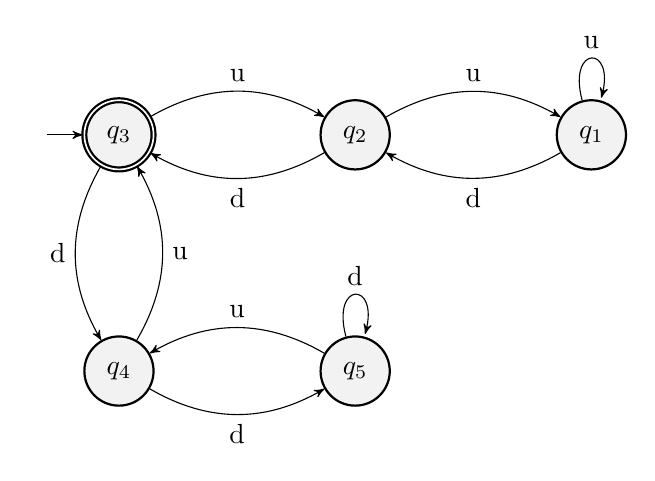
\begin{tikzpicture}
            \node[state, initial, accepting] (q3) {$q_3$};
            \node[state, right of=q3] (q2) {$q_2$};
            \node[state, right of=q2] (q1) {$q_1$};
            \node[state, below of=q3] (q4) {$q_4$};
            \node[state, right of=q4] (q5) {$q_5$};  
            \draw
                (q1) edge[loop above] node{u} (q1)
                (q1) edge[bend left, below] node{d} (q2)
                (q3) edge[bend left, above] node{u} (q2)
                (q3) edge[bend right, left] node{d} (q4)
                (q2) edge[bend left,  above] node{u} (q1)
                (q2) edge[bend left,  below] node{d} (q3)
                (q4) edge[bend right, right] node{u} (q3)
                (q4) edge[bend right, below] node{d} (q5)
                (q5) edge[bend right, above] node{u} (q4)
                (q5) edge[loop above] node{d} (q5);
        \end{tikzpicture}
    \end{figure}
\end{proof}
\cleardoublepage
\begin{proof}{\textbf{1.4}}
    \begin{itemize}
        \item[\textbf{a.}] Let $M_1$ be a machine that checks if
        the input string has at least 3 a's then
        \begin{align*}
            M_1 = \{\{q_1, q_2, q_3, q_4\}, \{a,b\}, \delta_1, q_1, \{q_4\}\}
        \end{align*}
        where $\delta_1$ is 
        \begin{center}
        \begin{tabular}{l|ll}
                  & a     & b     \\ \hline
            $q_1$ & $q_2$ & $q_1$ \\
            $q_2$ & $q_3$ & $q_2$ \\
            $q_3$ & $q_4$ & $q_3$ \\
            $q_4$ & $q_4$ & $q_4$ \\
        \end{tabular}
        \end{center}
        Let also, $M_2$ be a machine that checks if the input string has
        at least 2 b's then
        \begin{align*}
            M_2 = \{\{q_1, q_2, q_3\}, \{a,b\}, \delta_2, q_1, \{q_3\}\}
        \end{align*}
        where $\delta_2$ is 
        \begin{center}
        \begin{tabular}{l|ll}
                  & a     & b     \\ \hline
            $q_1$ & $q_1$ & $q_2$ \\
            $q_2$ & $q_2$ & $q_3$ \\
            $q_3$ & $q_3$ & $q_3$ \\
        \end{tabular}
        \end{center}
        Now we combine both machines into $M$ defined as
        \begin{align*}
            M = \{Q, \{a,b\}, \delta, (q_1,q_1), \{(q_4, q_3)\}\}
        \end{align*}
        where $Q$ is 
        \begin{align*}
            Q =\{q_1, q_2, q_3, q_4\} \times \{q_1, q_2, q_3\}
        \end{align*}
        and $\delta$ is 
        \begin{center}
        \begin{tabular}{l|ll}
                  & a     & b     \\ \hline
            $(q_1, q_1)$ & $(q_2, q_1)$ & $(q_1, q_2)$ \\
            $(q_1, q_2)$ & $(q_2, q_2)$ & $(q_1, q_3)$ \\
            $(q_1, q_3)$ & $(q_2, q_3)$ & $(q_1, q_3)$ \\
            $(q_2, q_1)$ & $(q_3, q_1)$ & $(q_2, q_2)$ \\
            $(q_2, q_2)$ & $(q_3, q_2)$ & $(q_2, q_3)$ \\
            $(q_2, q_3)$ & $(q_3, q_3)$ & $(q_2, q_3)$ \\
            $(q_3, q_1)$ & $(q_4, q_1)$ & $(q_3, q_2)$ \\
            $(q_3, q_2)$ & $(q_4, q_2)$ & $(q_3, q_3)$ \\
            $(q_3, q_3)$ & $(q_4, q_3)$ & $(q_3, q_3)$ \\
            $(q_4, q_1)$ & $(q_4, q_1)$ & $(q_4, q_2)$ \\
            $(q_4, q_2)$ & $(q_4, q_2)$ & $(q_4, q_3)$ \\
            $(q_4, q_3)$ & $(q_4, q_3)$ & $(q_4, q_3)$ \\
        \end{tabular}
        \end{center}
        Finally, the state diagram for this machine is given by
        \begin{figure}[H]
            \centering % centers the figure
            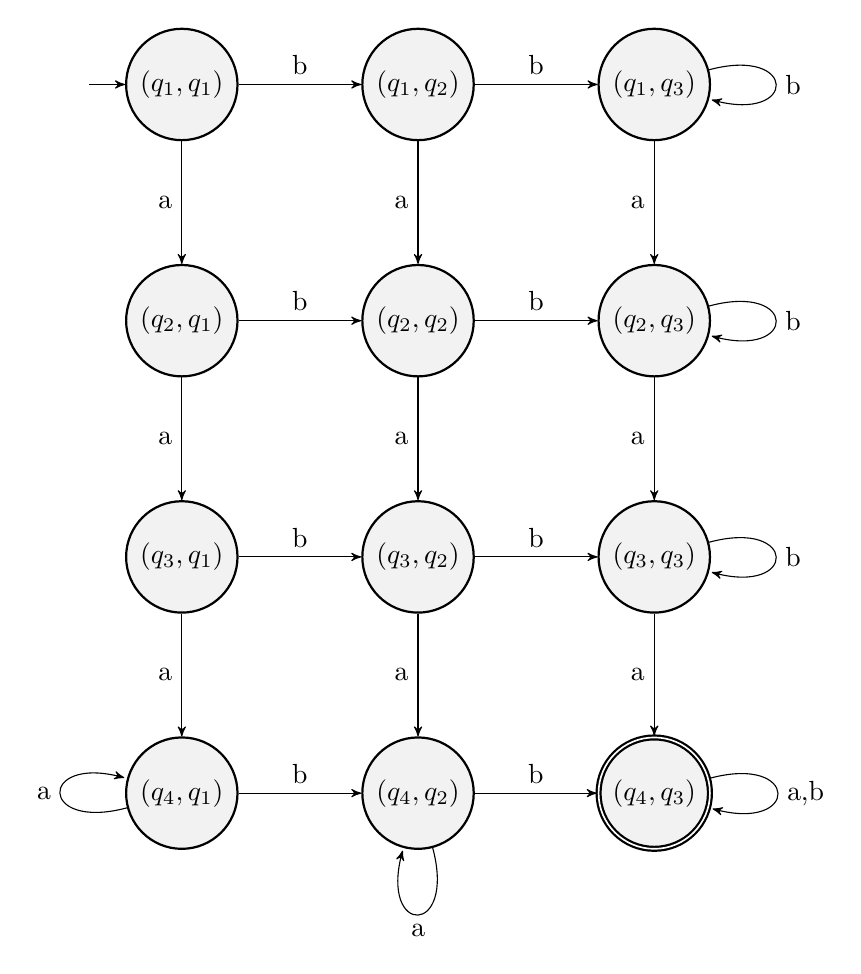
\begin{tikzpicture}
                \node[state, initial] (q1_q1) {$(q_1,q_1)$};
                \node[state, right of=q1_q1] (q1_q2) {$(q_1, q_2)$};
                \node[state, right of=q1_q2] (q1_q3) {$(q_1, q_3)$};

                \node[state, below of=q1_q1] (q2_q1) {$(q_2, q_1)$};
                \node[state, right of=q2_q1] (q2_q2) {$(q_2, q_2)$};
                \node[state, right of=q2_q2] (q2_q3) {$(q_2, q_3)$};

                \node[state, below of=q2_q1] (q3_q1) {$(q_3, q_1)$};
                \node[state, right of=q3_q1] (q3_q2) {$(q_3, q_2)$};
                \node[state, right of=q3_q2] (q3_q3) {$(q_3, q_3)$};

                \node[state, below of=q3_q1] (q4_q1) {$(q_4, q_1)$};
                \node[state, right of=q4_q1] (q4_q2) {$(q_4, q_2)$};
                \node[state, right of=q4_q2, accepting] (q4_q3) {$(q_4, q_3)$};

                \draw
                    (q1_q1) edge[left] node{a} (q2_q1)
                    (q1_q1) edge[above] node{b} (q1_q2)
                    (q1_q2) edge[ left] node{a} (q2_q2)
                    (q1_q2) edge[above] node{b} (q1_q3)
                    (q1_q3) edge[left] node{a} (q2_q3)
                    (q1_q3) edge[loop right] node{b} (q1_q3)
                    (q2_q1) edge[left] node{a} (q3_q1)
                    (q2_q1) edge[above] node{b} (q2_q2)
                    (q2_q2) edge[left] node{a} (q3_q2)
                    (q2_q2) edge[above] node{b} (q2_q3)
                    (q2_q3) edge[left] node{a} (q3_q3)
                    (q2_q3) edge[loop right] node{b} (q2_q2)
                    (q3_q1) edge[left] node{a} (q4_q1)
                    (q3_q1) edge[above] node{b} (q3_q2)
                    (q3_q2) edge[left] node{a} (q4_q2)
                    (q3_q2) edge[above] node{b} (q3_q3)
                    (q3_q3) edge[left] node{a} (q4_q3)
                    (q3_q3) edge[loop right] node{b} (q3_q3)
                    (q4_q1) edge[loop left] node{a} (q4_q1)
                    (q4_q1) edge[above] node{b} (q4_q2)
                    (q4_q2) edge[loop below] node{a} (q4_q2)
                    (q4_q2) edge[above] node{b} (q4_q3)
                    (q4_q3) edge[loop right] node{a,b} (q4_q3);
                \end{tikzpicture}
        \end{figure}
        \item[\textbf{b.}] Let $M_1$ be a machine that checks if
        the input string has exactly 2 a's then
        \begin{align*}
            M_1 = \{\{q_1, q_2, q_3, q_4\}, \{a,b\}, \delta_1, q_1, \{q_3\}\}
        \end{align*}
        where $\delta_1$ is 
        \begin{center}
        \begin{tabular}{l|ll}
                  & a     & b     \\ \hline
            $q_1$ & $q_2$ & $q_1$ \\
            $q_2$ & $q_3$ & $q_2$ \\
            $q_3$ & $q_4$ & $q_3$ \\
            $q_4$ & $q_4$ & $q_4$ \\
        \end{tabular}
        \end{center}
        Let us take $M_2$ as defined in part \textbf{a.}
        Now we combine both machines into $M$ defined as
        \begin{align*}
            M = \{Q, \{a,b\}, \delta, (q_1,q_1), \{(q_3, q_3)\}\}
        \end{align*}
        where $Q$ is 
        \begin{align*}
            Q =\{q_1, q_2, q_3, q_4\} \times \{q_1, q_2, q_3\}
        \end{align*}
        and $\delta$ is 
        \begin{center}
        \begin{tabular}{l|ll}
                  & a     & b     \\ \hline
            $(q_1, q_1)$ & $(q_2, q_1)$ & $(q_1, q_2)$ \\
            $(q_1, q_2)$ & $(q_2, q_2)$ & $(q_1, q_3)$ \\
            $(q_1, q_3)$ & $(q_2, q_3)$ & $(q_1, q_3)$ \\
            $(q_2, q_1)$ & $(q_3, q_1)$ & $(q_2, q_2)$ \\
            $(q_2, q_2)$ & $(q_3, q_2)$ & $(q_2, q_3)$ \\
            $(q_2, q_3)$ & $(q_3, q_3)$ & $(q_2, q_3)$ \\
            $(q_3, q_1)$ & $(q_4, q_1)$ & $(q_3, q_2)$ \\
            $(q_3, q_2)$ & $(q_4, q_2)$ & $(q_3, q_3)$ \\
            $(q_3, q_3)$ & $(q_4, q_3)$ & $(q_3, q_3)$ \\
            $(q_4, q_1)$ & $(q_4, q_1)$ & $(q_4, q_2)$ \\
            $(q_4, q_2)$ & $(q_4, q_2)$ & $(q_4, q_3)$ \\
            $(q_4, q_3)$ & $(q_4, q_3)$ & $(q_4, q_3)$ \\
        \end{tabular}
        \end{center}
        Finally, the state diagram for this machine is given by
        \begin{figure}[H]
            \centering % centers the figure
            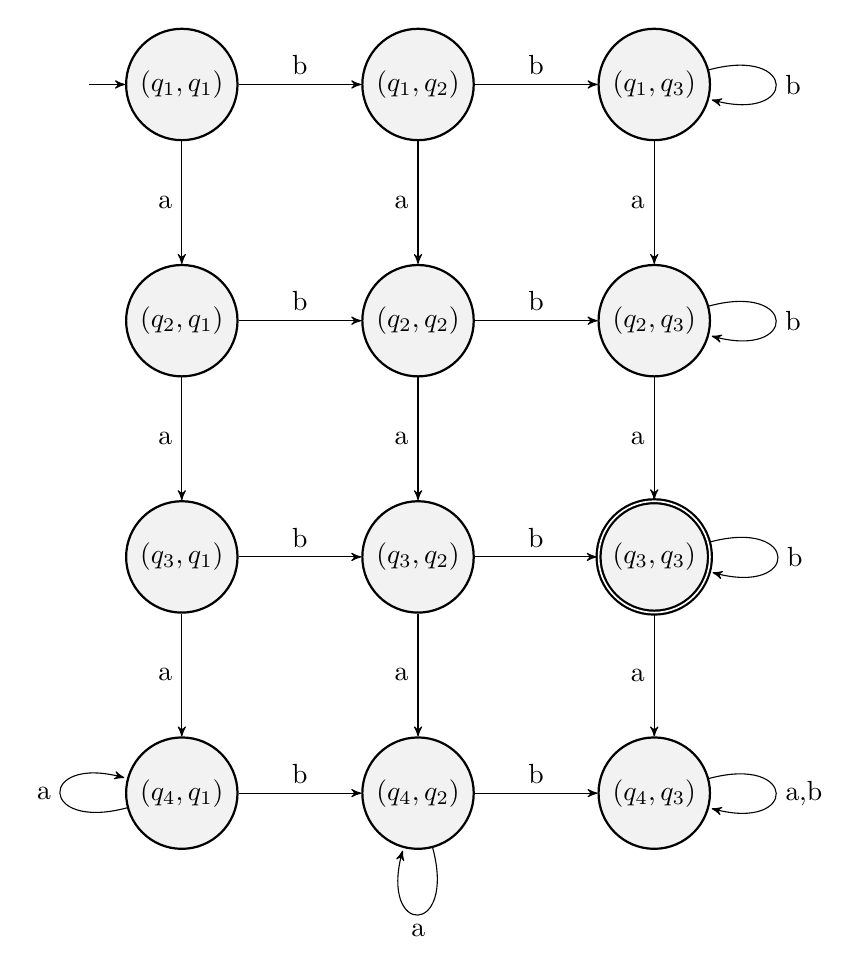
\begin{tikzpicture}
                \node[state, initial] (q1_q1) {$(q_1,q_1)$};
                \node[state, right of=q1_q1] (q1_q2) {$(q_1, q_2)$};
                \node[state, right of=q1_q2] (q1_q3) {$(q_1, q_3)$};

                \node[state, below of=q1_q1] (q2_q1) {$(q_2, q_1)$};
                \node[state, right of=q2_q1] (q2_q2) {$(q_2, q_2)$};
                \node[state, right of=q2_q2] (q2_q3) {$(q_2, q_3)$};

                \node[state, below of=q2_q1] (q3_q1) {$(q_3, q_1)$};
                \node[state, right of=q3_q1] (q3_q2) {$(q_3, q_2)$};
                \node[state, right of=q3_q2, accepting] (q3_q3) {$(q_3, q_3)$};

                \node[state, below of=q3_q1] (q4_q1) {$(q_4, q_1)$};
                \node[state, right of=q4_q1] (q4_q2) {$(q_4, q_2)$};
                \node[state, right of=q4_q2] (q4_q3) {$(q_4, q_3)$};

                \draw
                    (q1_q1) edge[left] node{a} (q2_q1)
                    (q1_q1) edge[above] node{b} (q1_q2)
                    (q1_q2) edge[ left] node{a} (q2_q2)
                    (q1_q2) edge[above] node{b} (q1_q3)
                    (q1_q3) edge[left] node{a} (q2_q3)
                    (q1_q3) edge[loop right] node{b} (q1_q3)
                    (q2_q1) edge[left] node{a} (q3_q1)
                    (q2_q1) edge[above] node{b} (q2_q2)
                    (q2_q2) edge[left] node{a} (q3_q2)
                    (q2_q2) edge[above] node{b} (q2_q3)
                    (q2_q3) edge[left] node{a} (q3_q3)
                    (q2_q3) edge[loop right] node{b} (q2_q2)
                    (q3_q1) edge[left] node{a} (q4_q1)
                    (q3_q1) edge[above] node{b} (q3_q2)
                    (q3_q2) edge[left] node{a} (q4_q2)
                    (q3_q2) edge[above] node{b} (q3_q3)
                    (q3_q3) edge[left] node{a} (q4_q3)
                    (q3_q3) edge[loop right] node{b} (q3_q3)
                    (q4_q1) edge[loop left] node{a} (q4_q1)
                    (q4_q1) edge[above] node{b} (q4_q2)
                    (q4_q2) edge[loop below] node{a} (q4_q2)
                    (q4_q2) edge[above] node{b} (q4_q3)
                    (q4_q3) edge[loop right] node{a,b} (q4_q3);
                \end{tikzpicture}
        \end{figure}
        \cleardoublepage
        \item[\textbf{c.}] Let $M_1$ be a machine that checks if
        the input string an even number of a's then
        \begin{align*}
            M_1 = \{\{q_1, q_2\}, \{a,b\}, \delta_1, q_1, \{q_1\}\}
        \end{align*}
        where $\delta_1$ is 
        \begin{center}
        \begin{tabular}{l|ll}
                  & a     & b     \\ \hline
            $q_1$ & $q_2$ & $q_1$ \\
            $q_2$ & $q_1$ & $q_2$ \\
        \end{tabular}
        \end{center}
        Let also, $M_2$ be a machine that checks if the input string has
        one or two b's then
        \begin{align*}
            M_2 = \{\{q_1, q_2, q_3, q_4\}, \{a,b\}, \delta_2, q_1, \{q_2, q_3\}\}
        \end{align*}
        where $\delta_2$ is 
        \begin{center}
        \begin{tabular}{l|ll}
                  & a     & b     \\ \hline
            $q_1$ & $q_1$ & $q_2$ \\
            $q_2$ & $q_2$ & $q_3$ \\
            $q_3$ & $q_3$ & $q_4$ \\
            $q_4$ & $q_4$ & $q_4$ \\
        \end{tabular}
        \end{center}
        Now we combine both machines into $M$ defined as
        \begin{align*}
            M = \{Q, \{a,b\}, \delta, (q_1,q_1), \{(q_1, q_2), (q_1, q_3)\}\}
        \end{align*}
        where $Q$ is 
        \begin{align*}
            Q =\{q_1, q_2\} \times \{q_1, q_2, q_3, q_4\}
        \end{align*}
        and $\delta$ is 
        \begin{center}
        \begin{tabular}{l|ll}
                  & a     & b     \\ \hline
            $(q_1, q_1)$ & $(q_2, q_1)$ & $(q_1, q_2)$ \\
            $(q_1, q_2)$ & $(q_2, q_2)$ & $(q_1, q_3)$ \\
            $(q_1, q_3)$ & $(q_2, q_3)$ & $(q_1, q_4)$ \\
            $(q_1, q_4)$ & $(q_2, q_4)$ & $(q_1, q_4)$ \\
            $(q_2, q_1)$ & $(q_1, q_1)$ & $(q_2, q_2)$ \\
            $(q_2, q_2)$ & $(q_1, q_2)$ & $(q_2, q_3)$ \\
            $(q_2, q_3)$ & $(q_1, q_3)$ & $(q_2, q_4)$ \\
            $(q_2, q_4)$ & $(q_1, q_4)$ & $(q_2, q_4)$ \\
        \end{tabular}
        \end{center}
        Finally, the state diagram for this machine is given by
        \begin{figure}[H]
            \centering % centers the figure
            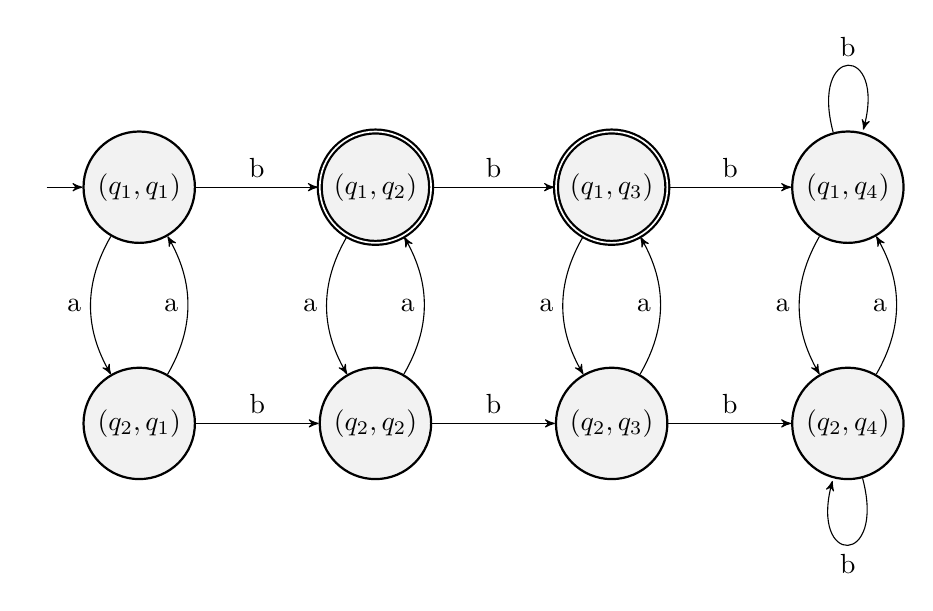
\begin{tikzpicture}
                \node[state, initial] (q1_q1) {$(q_1,q_1)$};
                \node[state, right of=q1_q1, accepting] (q1_q2) {$(q_1, q_2)$};
                \node[state, right of=q1_q2, accepting] (q1_q3) {$(q_1, q_3)$};
                \node[state, right of=q1_q3] (q1_q4) {$(q_1, q_4)$};

                \node[state, below of=q1_q1] (q2_q1) {$(q_2, q_1)$};
                \node[state, right of=q2_q1] (q2_q2) {$(q_2, q_2)$};
                \node[state, right of=q2_q2] (q2_q3) {$(q_2, q_3)$};
                \node[state, right of=q2_q3] (q2_q4) {$(q_2, q_4)$};
                \draw
                    (q1_q1) edge[bend right, left] node{a} (q2_q1)
                    (q1_q1) edge[above] node{b} (q1_q2)
                    (q1_q2) edge[bend right, left] node{a} (q2_q2)
                    (q1_q2) edge[above] node{b} (q1_q3)
                    (q1_q3) edge[bend right, left] node{a} (q2_q3)
                    (q1_q3) edge[above] node{b} (q1_q4)
                    (q1_q4) edge[bend right, left] node{a} (q2_q4)
                    (q1_q4) edge[loop above] node{b} (q1_q4)
                    %
                    (q2_q1) edge[bend right, left] node{a} (q1_q1)
                    (q2_q1) edge[above] node{b} (q2_q2)
                    (q2_q2) edge[bend right, left] node{a} (q1_q2)
                    (q2_q2) edge[above] node{b} (q2_q3)
                    (q2_q3) edge[bend right, left] node{a} (q1_q3)
                    (q2_q3) edge[above] node{b} (q2_q4)
                    (q2_q4) edge[bend right, left] node{a} (q1_q4)
                    (q2_q4) edge[loop below] node{b} (q2_q4);
                \end{tikzpicture}
        \end{figure}
        \item[\textbf{d.}] Let $M_1$ be the machine defined in part \textbf{c}.
        Let also, $M_2$ be a machine that checks if the input string has
        each a followed by at least one b then
        \begin{align*}
            M_2 = \{\{q_1, q_2, q_3\}, \{a,b\}, \delta_2, q_1, \{q_1\}\}
        \end{align*}
        where $\delta_2$ is 
        \begin{center}
        \begin{tabular}{l|ll}
                  & a     & b     \\ \hline
            $q_1$ & $q_2$ & $q_1$ \\
            $q_2$ & $q_3$ & $q_1$ \\
            $q_3$ & $q_3$ & $q_3$ \\
        \end{tabular}
        \end{center}
        Now we combine both machines into $M$ defined as
        \begin{align*}
            M = \{Q, \{a,b\}, \delta, (q_1,q_1), \{(q_1, q_1)\}\}
        \end{align*}
        where $Q$ is 
        \begin{align*}
            Q =\{q_1, q_2\} \times \{q_1, q_2, q_3\}
        \end{align*}
        and $\delta$ is 
        \begin{center}
        \begin{tabular}{l|ll}
                  & a     & b     \\ \hline
            $(q_1, q_1)$ & $(q_2, q_2)$ & $(q_1, q_1)$ \\
            $(q_1, q_2)$ & $(q_2, q_3)$ & $(q_1, q_1)$ \\
            $(q_1, q_3)$ & $(q_2, q_3)$ & $(q_1, q_3)$ \\
            $(q_2, q_1)$ & $(q_1, q_2)$ & $(q_2, q_1)$ \\
            $(q_2, q_2)$ & $(q_1, q_3)$ & $(q_2, q_1)$ \\
            $(q_2, q_3)$ & $(q_1, q_3)$ & $(q_2, q_3)$ \\
        \end{tabular}
        \end{center}
        Finally, the state diagram for this machine is given by
        \begin{figure}[H]
            \centering % centers the figure
            \begin{tikzpicture}
                \node[state, initial, accepting] (q1_q1) {$(q_1,q_1)$};
                \node[state, right of=q1_q1] (q1_q2) {$(q_1, q_2)$};
                \node[state, below of=q2_q3, right of=q2_q2] (q1_q3) {$(q_1, q_3)$};

                \node[state, below of=q1_q2] (q2_q1) {$(q_2, q_1)$};
                \node[state, below of=q2_q1] (q2_q2) {$(q_2, q_2)$};
                \node[state, right of=q1_q2] (q2_q3) {$(q_2, q_3)$};
                \draw
                    (q1_q1) edge[right] node{a} (q2_q2)
                    (q1_q1) edge[loop above] node{b} (q1_q1)
                    (q1_q2) edge[right, above] node{a} (q2_q3)
                    (q1_q2) edge[above] node{b} (q1_q1)
                    (q1_q3) edge[left] node{a} (q2_q3)
                    (q1_q3) edge[loop right] node{b} (q1_q3)
                    % 
                    (q2_q1) edge[left] node{a} (q1_q2)
                    (q2_q1) edge[loop right] node{b} (q2_q1)
                    (q2_q2) edge[above] node{a} (q1_q3)
                    (q2_q2) edge[right] node{b} (q2_q1)
                    (q2_q3) edge[bend left, left] node{a} (q1_q3)
                    (q2_q3) edge[loop above, above] node{b} (q2_q3)
                    ;
                \end{tikzpicture}
        \end{figure}
        \item[\textbf{e.}] Let $M_1$ be a machine that checks if
        the input string starts with an a then
        \begin{align*}
            M_1 = \{\{q_1, q_2, q_3\}, \{a,b\}, \delta_1, q_1, \{q_2\}\}
        \end{align*}
        where $\delta_1$ is 
        \begin{center}
        \begin{tabular}{l|ll}
                  & a     & b     \\ \hline
            $q_1$ & $q_2$ & $q_3$ \\
            $q_2$ & $q_2$ & $q_2$ \\
            $q_3$ & $q_3$ & $q_3$ \\
        \end{tabular}
        \end{center}
        Let also, $M_2$ be a machine that checks if the input string has
        at most one b then
        \begin{align*}
            M_2 = \{\{q_1, q_2, q_3\}, \{a,b\}, \delta_2, q_1, \{q_2\}\}
        \end{align*}
        where $\delta_2$ is 
        \begin{center}
        \begin{tabular}{l|ll}
                  & a     & b     \\ \hline
            $q_1$ & $q_1$ & $q_2$ \\
            $q_2$ & $q_2$ & $q_3$ \\
            $q_3$ & $q_3$ & $q_3$ \\
        \end{tabular}
        \end{center}
        Now we combine both machines into $M$ defined as
        \begin{align*}
            M = \{Q, \{a,b\}, \delta, (q_1,q_1), \{(q_2, q_2)\}\}
        \end{align*}
        where $Q$ is 
        \begin{align*}
            Q =\{q_1, q_2, q_3\} \times \{q_1, q_2, q_3\}
        \end{align*}
        and $\delta$ is 
        \begin{center}
        \begin{tabular}{l|ll}
                  & a     & b     \\ \hline
            $(q_1, q_1)$ & $(q_2, q_1)$ & $(q_3, q_2)$ \\
            $(q_1, q_2)$ & $(q_2, q_2)$ & $(q_3, q_3)$ \\
            $(q_1, q_3)$ & $(q_2, q_3)$ & $(q_3, q_3)$ \\
            $(q_2, q_1)$ & $(q_2, q_1)$ & $(q_2, q_2)$ \\
            $(q_2, q_2)$ & $(q_2, q_2)$ & $(q_2, q_3)$ \\
            $(q_2, q_3)$ & $(q_2, q_3)$ & $(q_2, q_3)$ \\
            $(q_3, q_1)$ & $(q_3, q_1)$ & $(q_3, q_2)$ \\
            $(q_3, q_2)$ & $(q_3, q_2)$ & $(q_3, q_3)$ \\
            $(q_3, q_3)$ & $(q_3, q_3)$ & $(q_3, q_3)$ \\
        \end{tabular}
        \end{center}
        Finally, the state diagram for this machine is given by
        \begin{figure}[H]
            \centering % centers the figure
            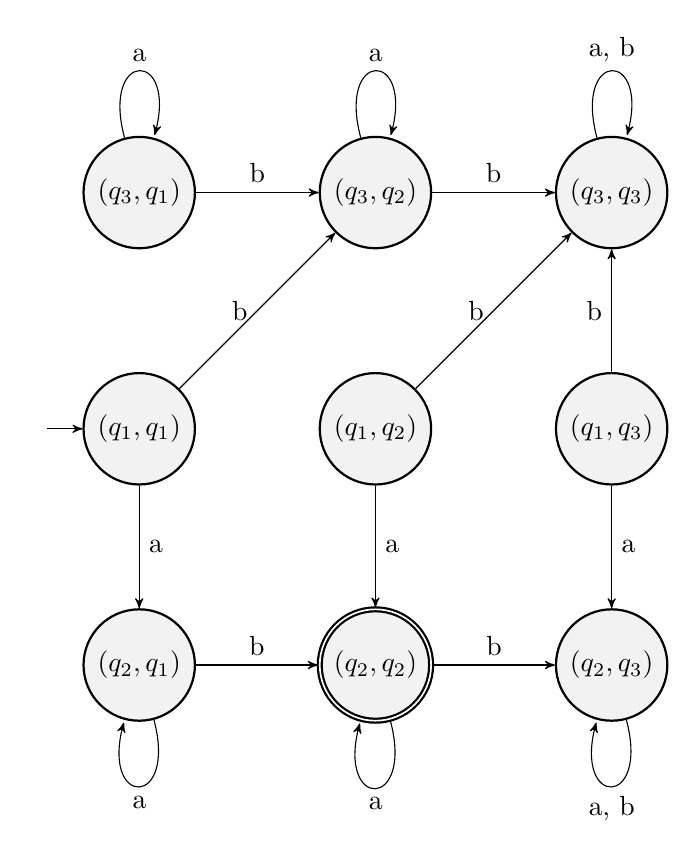
\begin{tikzpicture}
                \node[state, initial] (q1_q1) {$(q_1, q_1)$};
                \node[state, right of=q1_q1] (q1_q2) {$(q_1, q_2)$};
                \node[state, right of=q1_q2] (q1_q3) {$(q_1, q_3)$};

                \node[state, below of=q1_q1] (q2_q1) {$(q_2, q_1)$};
                \node[state, right of=q2_q1, accepting] (q2_q2) {$(q_2, q_2)$};
                \node[state, right of=q2_q2] (q2_q3) {$(q_2, q_3)$};

                \node[state, above of=q1_q1] (q3_q1) {$(q_3, q_1)$};
                \node[state, right of=q3_q1] (q3_q2) {$(q_3, q_2)$};
                \node[state, right of=q3_q2] (q3_q3) {$(q_3, q_3)$};
                \draw
                    (q1_q1) edge[right] node{a} (q2_q1)
                    (q1_q1) edge[left] node{b} (q3_q2)
                    (q1_q2) edge[right] node{a} (q2_q2)
                    (q1_q2) edge[left] node{b} (q3_q3)
                    (q1_q3) edge[right] node{a} (q2_q3)
                    (q1_q3) edge[left] node{b} (q3_q3)
                    %
                    (q2_q1) edge[loop below] node{a} (q2_q1)
                    (q2_q1) edge[above] node{b} (q2_q2)
                    (q2_q2) edge[loop below] node{a} (q2_q2)
                    (q2_q2) edge[above] node{b} (q2_q3)
                    (q2_q3) edge[loop below] node{a, b} (q2_q3)
                    %
                    (q3_q1) edge[loop above] node{a} (q3_q1)
                    (q3_q1) edge[above] node{b} (q3_q2)
                    (q3_q2) edge[loop above] node{a} (q3_q2)
                    (q3_q2) edge[above] node{b} (q3_q3)
                    (q3_q3) edge[loop above] node{a, b} (q3_q3)
                    ;
                \end{tikzpicture}
        \end{figure}
        \cleardoublepage
        \item[\textbf{f.}] Let $M_1$ be a machine that checks if
        the input string has an odd number of a's then $M_1$ is defined as
        \begin{figure}[H]
            \centering % centers the figure
            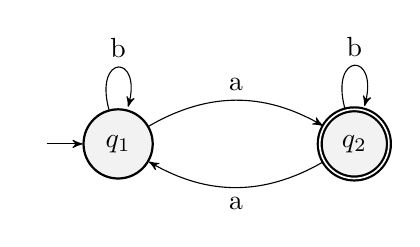
\begin{tikzpicture}
                \node[state, initial] (q1) {$q_1$};
                \node[state, right of=q1, accepting] (q2) {$q_2$};
                \draw
                    (q1) edge[bend left, above] node{a} (q2)
                    (q1) edge[loop above] node{b} (q1)
                    (q2) edge[bend left, below] node{a} (q1)
                    (q2) edge[loop above] node{b} (q2)
                    ;
                \end{tikzpicture}
        \end{figure}
        Let also, $M_2$ be a machine that checks if the input string ends
        with a b then $M_2$ is defined as
        \begin{figure}[H]
            \centering % centers the figure
            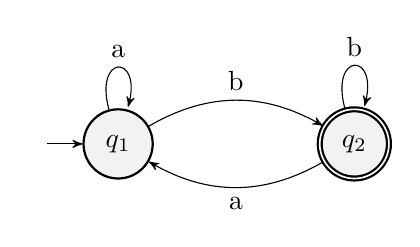
\begin{tikzpicture}
                \node[state, initial] (q1) {$q_1$};
                \node[state, right of=q1, accepting] (q2) {$q_2$};
                \draw
                    (q1) edge[loop above] node{a} (q1)
                    (q1) edge[bend left, above] node{b} (q2)
                    (q2) edge[bend left, below] node{a} (q1)
                    (q2) edge[loop above] node{b} (q2)
                    ;
                \end{tikzpicture}
        \end{figure}
        Now we combine both machines into $M$ defined as
        \begin{figure}[H]
            \centering % centers the figure
            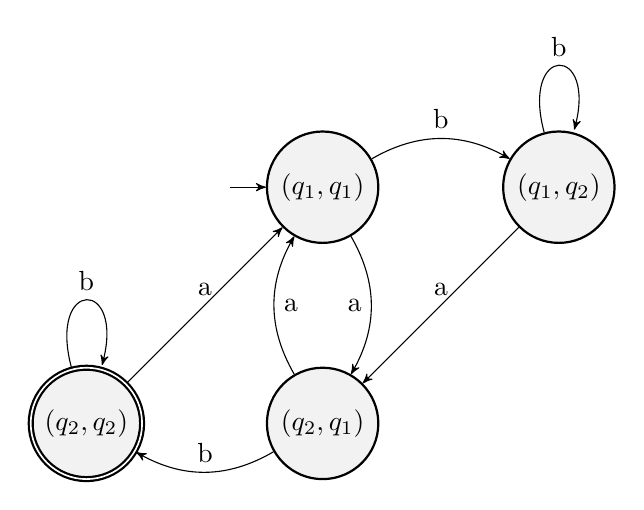
\begin{tikzpicture}
                \node[state, initial] (q1_q1) {$(q_1, q_1)$};
                \node[state, right of=q1_q1] (q1_q2) {$(q_1, q_2)$};
                \node[state, below of=q1_q1] (q2_q1) {$(q_2, q_1)$};
                \node[state, left of=q2_q1, accepting] (q2_q2) {$(q_2, q_2)$};
                \draw
                    (q1_q1) edge[bend left, left] node{a} (q2_q1)
                    (q1_q1) edge[bend left, above] node{b} (q1_q2)
                    (q1_q2) edge[above] node{a} (q2_q1)
                    (q1_q2) edge[loop above] node{b} (q1_q2)
                    (q2_q1) edge[bend left, right] node{a} (q1_q1)
                    (q2_q1) edge[bend left, above] node{b} (q2_q2)
                    (q2_q2) edge[above] node{a} (q1_q1)
                    (q2_q2) edge[loop above] node{b} (q2_q2)
                    ;
                \end{tikzpicture}
        \end{figure}
        \cleardoublepage
        \item[\textbf{g.}] Let $M_1$ be a machine that checks if
        the input string has an even length then $M_1$ is defined as
        \begin{figure}[H]
            \centering % centers the figure
            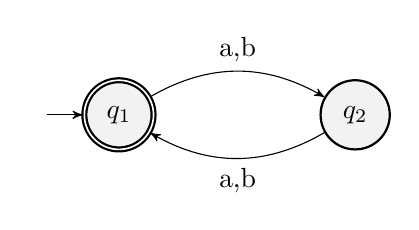
\begin{tikzpicture}
                \node[state, initial, accepting] (q1) {$q_1$};
                \node[state, right of=q1] (q2) {$q_2$};
                \draw
                    (q1) edge[bend left, above] node{a,b} (q2)
                    (q2) edge[bend left, below] node{a,b} (q1)
                    ;
                \end{tikzpicture}
        \end{figure}
        Let also, $M_2$ be a machine that checks if the input string has
        an odd number of a's then $M_2$ is defined as
        \begin{figure}[H]
            \centering % centers the figure
            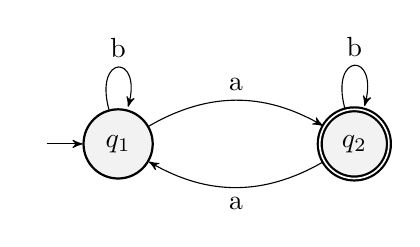
\begin{tikzpicture}
                \node[state, initial] (q1) {$q_1$};
                \node[state, right of=q1, accepting] (q2) {$q_2$};
                \draw
                    (q1) edge[bend left, above] node{a} (q2)
                    (q1) edge[loop above] node{b} (q1)
                    (q2) edge[bend left, below] node{a} (q1)
                    (q2) edge[loop above] node{b} (q2)
                    ;
                \end{tikzpicture}
        \end{figure}
        Now we combine both machines into $M$ defined as
        \begin{figure}[H]
            \centering % centers the figure
            \begin{tikzpicture}
                \node[state, initial] (q1_q1) {$(q_1, q_1)$};
                \node[state, right of=q2_q1, accepting] (q1_q2) {$(q_1, q_2)$};
                \node[state, right of=q1_q1] (q2_q1) {$(q_2, q_1)$};
                \node[state, below of=q1_q1] (q2_q2) {$(q_2, q_2)$};
                \draw
                    (q1_q1) edge[bend left, right] node{a} (q2_q2)
                    (q1_q1) edge[bend left, above] node{b} (q2_q1)
                    (q1_q2) edge[bend left, left] node{a} (q2_q1)
                    (q1_q2) edge[bend left, below] node{b} (q2_q2)
                    (q2_q1) edge[bend left, right] node{a} (q1_q2)
                    (q2_q1) edge[bend left, above] node{b} (q1_q1)
                    (q2_q2) edge[bend left, right] node{a} (q1_q1)
                    (q2_q2) edge[bend left, below] node{b} (q1_q2)
                    ;
                \end{tikzpicture}
        \end{figure}
    \end{itemize}
\end{proof}
\cleardoublepage
\begin{proof}{\textbf{1.5}}
    \begin{itemize}
        \item [\textbf{a.}] Let $M$ be a machine that checks if
        the input string contains the substring "ab" then $M$ is defined as
        \begin{figure}[H]
            \centering % centers the figure
            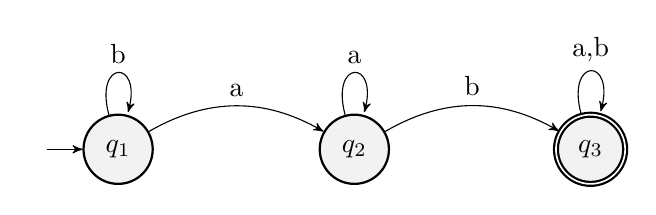
\begin{tikzpicture}
                \node[state, initial] (q1) {$q_1$};
                \node[state, right of=q1] (q2) {$q_2$};
                \node[state, right of=q2, accepting] (q3) {$q_3$};

                \draw
                    (q1) edge[bend left, above] node{a} (q2)
                    (q1) edge[loop above] node{b} (q1)
                    (q2) edge[bend left, above] node{b} (q3)
                    (q2) edge[loop above] node{a} (q1)
                    (q3) edge[loop above] node{a,b} (q3)
                    ;
                \end{tikzpicture}
        \end{figure}
        Then the complement of the machine $M$ is 
        \begin{figure}[H]
            \centering % centers the figure
            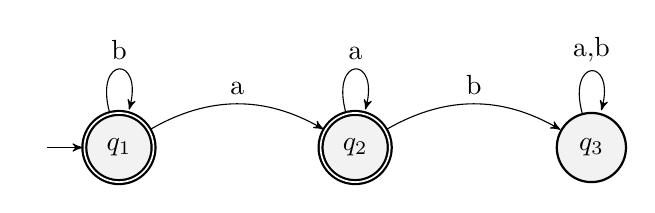
\begin{tikzpicture}
                \node[state, initial, accepting] (q1) {$q_1$};
                \node[state, right of=q1, accepting] (q2) {$q_2$};
                \node[state, right of=q2] (q3) {$q_3$};

                \draw
                    (q1) edge[bend left, above] node{a} (q2)
                    (q1) edge[loop above] node{b} (q1)
                    (q2) edge[bend left, above] node{b} (q3)
                    (q2) edge[loop above] node{a} (q1)
                    (q3) edge[loop above] node{a,b} (q3)
                    ;
                \end{tikzpicture}
        \end{figure}
        Since it will accept any string that doesn't contain the substring "ab".
        \item [\textbf{b.}] Let $M$ be a machine that checks if
        the input string contains the substring "baba" then $M$ is defined as
        \begin{figure}[H]
            \centering % centers the figure
            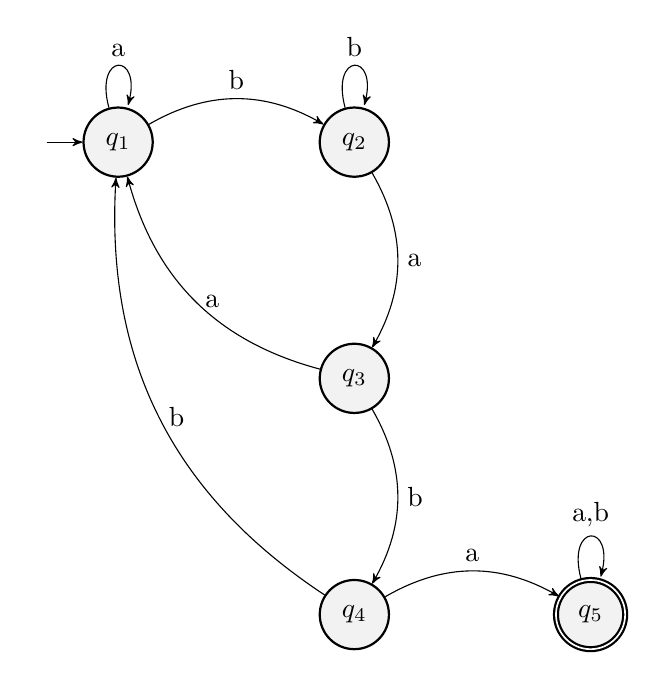
\begin{tikzpicture}
                \node[state, initial] (q1) {$q_1$};
                \node[state, right of=q1] (q2) {$q_2$};
                \node[state, below of=q2] (q3) {$q_3$};
                \node[state, below of=q3] (q4) {$q_4$};
                \node[state, right of=q4, accepting] (q5) {$q_5$};
                \draw
                    (q1) edge[bend left, above] node{b} (q2)
                    (q1) edge[loop above] node{a} (q1)
                    (q2) edge[bend left, right] node{a} (q3)
                    (q2) edge[loop above] node{b} (q1)
                    (q3) edge[bend left, right] node{b} (q4)
                    (q3) edge[bend left, right] node{a} (q1)
                    (q4) edge[bend left, right] node{b} (q1)
                    (q4) edge[bend left, above] node{a} (q5)
                    (q5) edge[loop above] node{a,b} (q5)
                    ;
                \end{tikzpicture}
        \end{figure}
        Then the complement of the machine $M$ is 
        \begin{figure}[H]
            \centering % centers the figure
            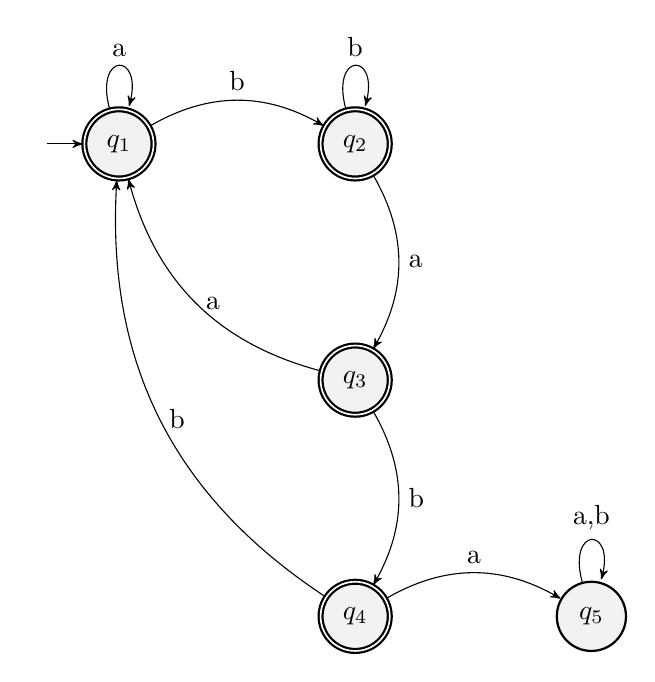
\begin{tikzpicture}
                \node[state, initial, accepting] (q1) {$q_1$};
                \node[state, right of=q1, accepting] (q2) {$q_2$};
                \node[state, below of=q2, accepting] (q3) {$q_3$};
                \node[state, below of=q3, accepting] (q4) {$q_4$};
                \node[state, right of=q4] (q5) {$q_5$};
                \draw
                    (q1) edge[bend left, above] node{b} (q2)
                    (q1) edge[loop above] node{a} (q1)
                    (q2) edge[bend left, right] node{a} (q3)
                    (q2) edge[loop above] node{b} (q1)
                    (q3) edge[bend left, right] node{b} (q4)
                    (q3) edge[bend left, right] node{a} (q1)
                    (q4) edge[bend left, right] node{b} (q1)
                    (q4) edge[bend left, above] node{a} (q5)
                    (q5) edge[loop above] node{a,b} (q5)
                    ;
                \end{tikzpicture}
        \end{figure}
        Since it will accept any string that doesn't contain the substring
        "baba".
\cleardoublepage
        \item [\textbf{c.}] Let $M$ be a machine that checks if
        the input string contains both the substring "ab" and "ba" then
        $M$ is defined as
        \begin{figure}[H]
            \centering
            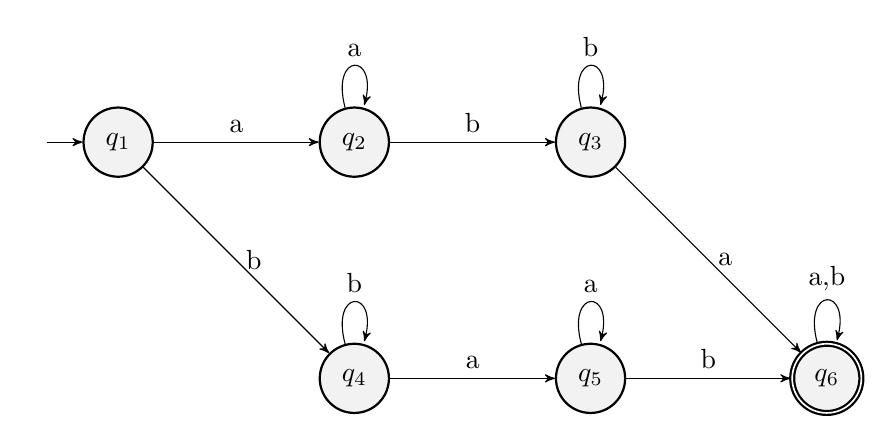
\begin{tikzpicture}
                \node[state, initial] (q1) {$q_1$};
                \node[state, right of=q1] (q2) {$q_2$};
                \node[state, right of=q2] (q3) {$q_3$};
                \node[state, below of=q2] (q4) {$q_4$};
                \node[state, right of=q4] (q5) {$q_5$};
                \node[state, right of=q5, accepting] (q6) {$q_6$};
                \draw
                    (q1) edge[above] node{a} (q2)
                    (q1) edge[right] node{b} (q4)
                    (q2) edge[loop above] node{a} (q2)
                    (q2) edge[above] node{b} (q3)
                    (q3) edge[right] node{a} (q6)
                    (q3) edge[loop above] node{b} (q3)
                    (q4) edge[above] node{a} (q5)
                    (q4) edge[loop above] node{b} (q4)
                    (q5) edge[loop above] node{a} (q5)
                    (q5) edge[above] node{b} (q6)
                    (q6) edge[loop above] node{a,b} (q6)
                    ;
                \end{tikzpicture}
        \end{figure}
        Then the complement of the machine $M$ is 
        \begin{figure}[H]
            \centering
            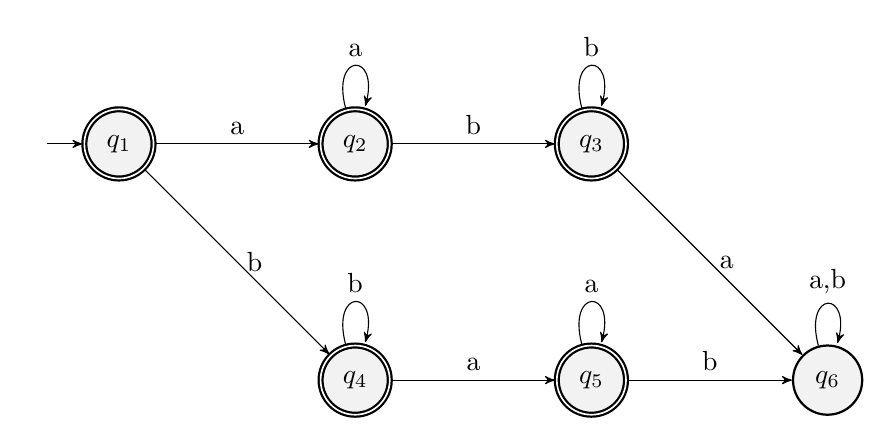
\begin{tikzpicture}
                \node[state, initial, accepting] (q1) {$q_1$};
                \node[state, right of=q1, accepting] (q2) {$q_2$};
                \node[state, right of=q2, accepting] (q3) {$q_3$};
                \node[state, below of=q2, accepting] (q4) {$q_4$};
                \node[state, right of=q4, accepting] (q5) {$q_5$};
                \node[state, right of=q5] (q6) {$q_6$};
                \draw
                    (q1) edge[above] node{a} (q2)
                    (q1) edge[right] node{b} (q4)
                    (q2) edge[loop above] node{a} (q2)
                    (q2) edge[above] node{b} (q3)
                    (q3) edge[right] node{a} (q6)
                    (q3) edge[loop above] node{b} (q3)
                    (q4) edge[above] node{a} (q5)
                    (q4) edge[loop above] node{b} (q4)
                    (q5) edge[loop above] node{a} (q5)
                    (q5) edge[above] node{b} (q6)
                    (q6) edge[loop above] node{a,b} (q6)
                    ;
                \end{tikzpicture}
        \end{figure}
    \cleardoublepage
        \item [\textbf{d.}] Let $M$ be a machine that checks if
        the input string is in $a^*b^*$ then $M$ is defined as
        \begin{figure}[H]
            \centering
            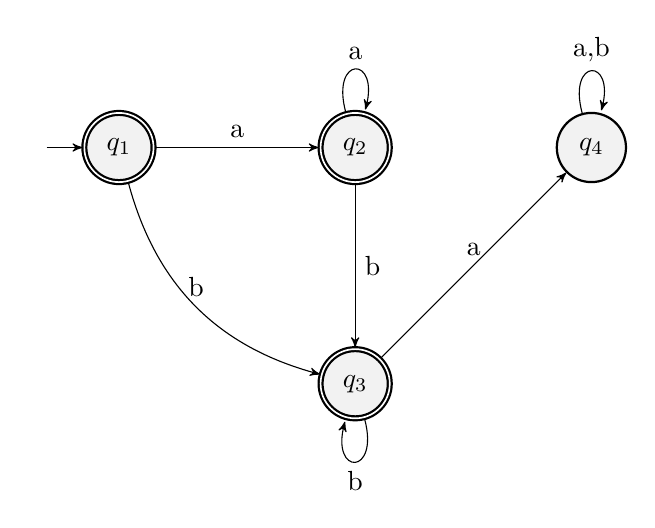
\begin{tikzpicture}
                \node[state, initial, accepting] (q1) {$q_1$};
                \node[state, right of=q1, accepting] (q2) {$q_2$};
                \node[state, below of=q2, accepting] (q3) {$q_3$};
                \node[state, right of=q2] (q4) {$q_4$};
                \draw
                    (q1) edge[above] node{a} (q2)
                    (q1) edge[above, bend right] node{b} (q3)
                    (q2) edge[loop above] node{a} (q2)
                    (q2) edge[right] node{b} (q3)
                    (q3) edge[loop below] node{b} (q3)
                    (q3) edge[above] node{a} (q4)
                    (q4) edge[loop above] node{a,b} (q4)
                    ;
                \end{tikzpicture}
        \end{figure}
        Then the complement of the machine $M$ is
        \begin{figure}[H]
            \centering
            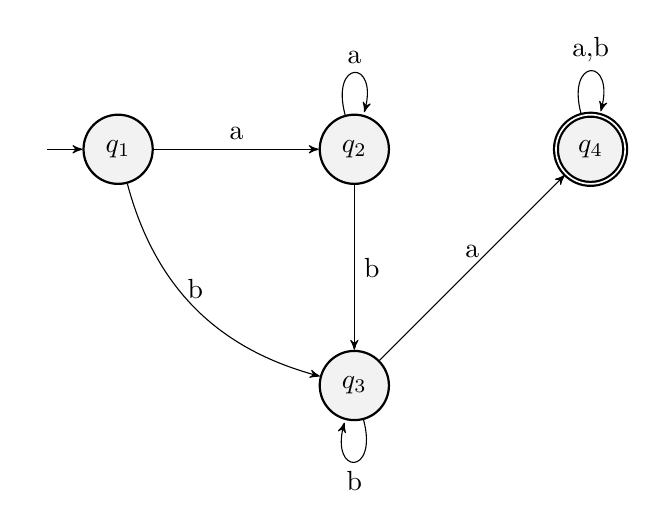
\begin{tikzpicture}
                \node[state, initial] (q1) {$q_1$};
                \node[state, right of=q1] (q2) {$q_2$};
                \node[state, below of=q2] (q3) {$q_3$};
                \node[state, right of=q2, accepting] (q4) {$q_4$};
                \draw
                    (q1) edge[above] node{a} (q2)
                    (q1) edge[above, bend right] node{b} (q3)
                    (q2) edge[loop above] node{a} (q2)
                    (q2) edge[right] node{b} (q3)
                    (q3) edge[loop below] node{b} (q3)
                    (q3) edge[above] node{a} (q4)
                    (q4) edge[loop above] node{a,b} (q4)
                    ;
                \end{tikzpicture}
        \end{figure}
    \cleardoublepage
        \item [\textbf{e.}] Let $M$ be a machine that checks if
        the input string is in $(ab^+)^*$ then $M$ is defined as
        \begin{figure}[H]
            \centering
            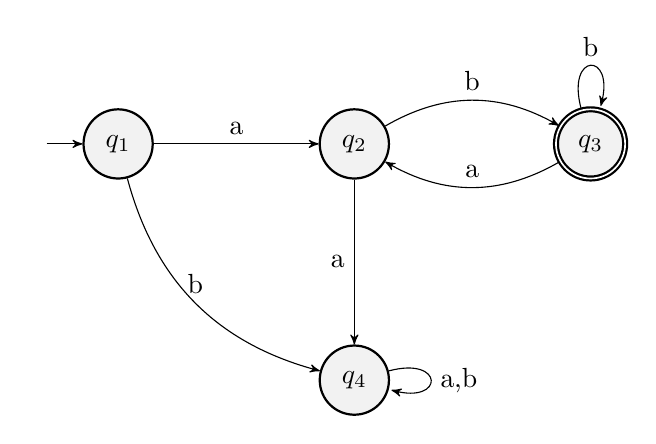
\begin{tikzpicture}
                \node[state, initial] (q1) {$q_1$};
                \node[state, right of=q1] (q2) {$q_2$};
                \node[state, right of=q2, accepting] (q3) {$q_3$};
                \node[state, below of=q2] (q4) {$q_4$};
                \draw
                    (q1) edge[above] node{a} (q2)
                    (q1) edge[above, bend right] node{b} (q4)
                    (q2) edge[left] node{a} (q4)
                    (q2) edge[above, bend left] node{b} (q3)
                    (q3) edge[above, bend left] node{a} (q2)
                    (q3) edge[loop above] node{b} (q3)
                    (q4) edge[loop right] node{a,b} (q4)
                    ;
                \end{tikzpicture}
        \end{figure}
        Then the complement of the machine $M$ is
        \begin{figure}[H]
            \centering
            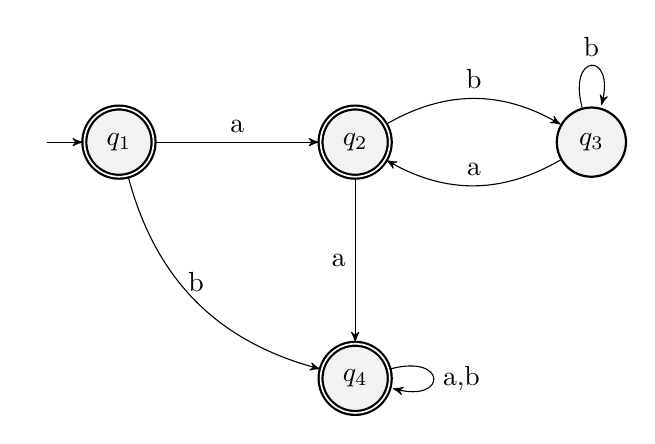
\begin{tikzpicture}
                \node[state, initial, accepting] (q1) {$q_1$};
                \node[state, right of=q1, accepting] (q2) {$q_2$};
                \node[state, right of=q2] (q3) {$q_3$};
                \node[state, below of=q2, accepting] (q4) {$q_4$};
                \draw
                    (q1) edge[above] node{a} (q2)
                    (q1) edge[above, bend right] node{b} (q4)
                    (q2) edge[left] node{a} (q4)
                    (q2) edge[above, bend left] node{b} (q3)
                    (q3) edge[above, bend left] node{a} (q2)
                    (q3) edge[loop above] node{b} (q3)
                    (q4) edge[loop right] node{a,b} (q4)
                    ;
                \end{tikzpicture}
        \end{figure}
        \cleardoublepage
        \item [\textbf{f.}] Let $M$ be a machine that checks if
        the input string is in $a^* \cup b^*$ then $M$ is defined as
        \begin{figure}[H]
            \centering
            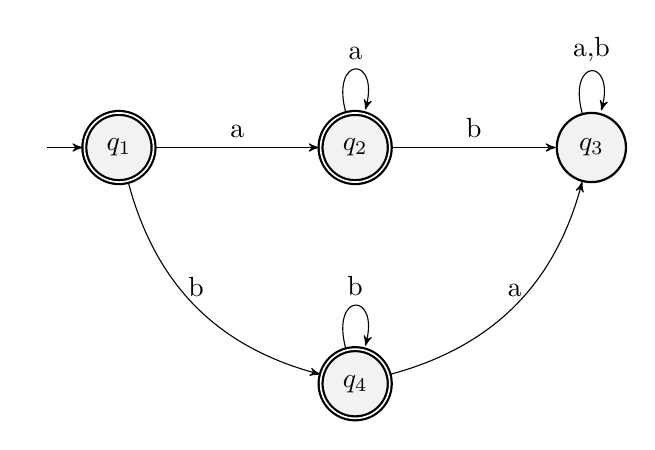
\begin{tikzpicture}
                \node[state, initial, accepting] (q1) {$q_1$};
                \node[state, right of=q1, accepting] (q2) {$q_2$};
                \node[state, right of=q2] (q3) {$q_3$};
                \node[state, below of=q2, accepting] (q4) {$q_4$};
                \draw
                    (q1) edge[above] node{a} (q2)
                    (q1) edge[above, bend right] node{b} (q4)
                    (q2) edge[loop above] node{a} (q2)
                    (q2) edge[above] node{b} (q3)
                    (q3) edge[loop above] node{a,b} (q3)
                    (q4) edge[above, bend right] node{a} (q3)
                    (q4) edge[loop above] node{b} (q4)
                    ;
                \end{tikzpicture}
        \end{figure}
        Then the complement of the machine $M$ is
        \begin{figure}[H]
            \centering
            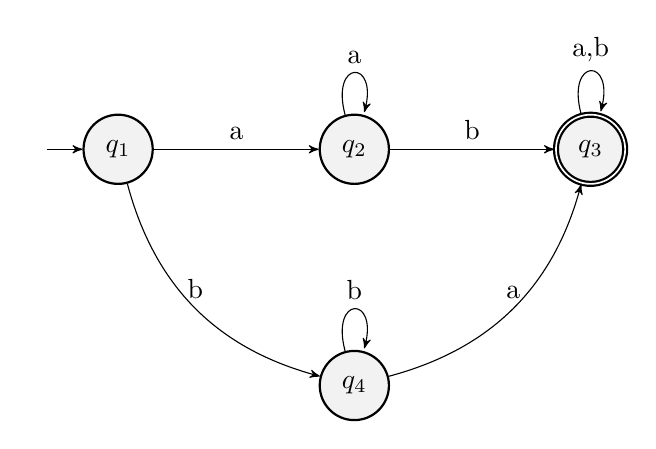
\begin{tikzpicture}
                \node[state, initial] (q1) {$q_1$};
                \node[state, right of=q1] (q2) {$q_2$};
                \node[state, right of=q2, accepting] (q3) {$q_3$};
                \node[state, below of=q2] (q4) {$q_4$};
                \draw
                    (q1) edge[above] node{a} (q2)
                    (q1) edge[above, bend right] node{b} (q4)
                    (q2) edge[loop above] node{a} (q2)
                    (q2) edge[above] node{b} (q3)
                    (q3) edge[loop above] node{a,b} (q3)
                    (q4) edge[above, bend right] node{a} (q3)
                    (q4) edge[loop above] node{b} (q4)
                    ;
                \end{tikzpicture}
        \end{figure}
    \cleardoublepage
        \item [\textbf{g.}] Let $M$ be a machine that checks if
        the input string contains exactly two a's then $M$ is defined as
        \begin{figure}[H]
            \centering
            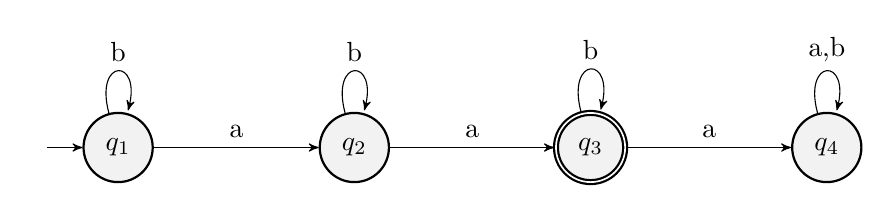
\begin{tikzpicture}
                \node[state, initial] (q1) {$q_1$};
                \node[state, right of=q1] (q2) {$q_2$};
                \node[state, right of=q2, accepting] (q3) {$q_3$};
                \node[state, right of=q3] (q4) {$q_4$};
                \draw
                    (q1) edge[above] node{a} (q2)
                    (q1) edge[loop above] node{b} (q1)
                    (q2) edge[above] node{a} (q3)
                    (q2) edge[loop above] node{b} (q2)
                    (q3) edge[above] node{a} (q4)
                    (q3) edge[loop above] node{b} (q3)
                    (q4) edge[loop above] node{a,b} (q4)
                    ;
                \end{tikzpicture}
        \end{figure}
        Then the complement of the machine $M$ is
        \begin{figure}[H]
            \centering
            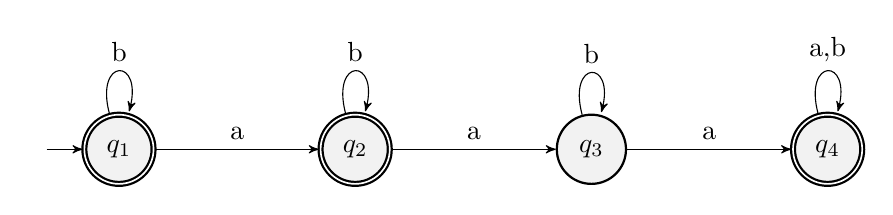
\begin{tikzpicture}
                \node[state, initial, accepting] (q1) {$q_1$};
                \node[state, right of=q1, accepting] (q2) {$q_2$};
                \node[state, right of=q2] (q3) {$q_3$};
                \node[state, right of=q3, accepting] (q4) {$q_4$};
                \draw
                    (q1) edge[above] node{a} (q2)
                    (q1) edge[loop above] node{b} (q1)
                    (q2) edge[above] node{a} (q3)
                    (q2) edge[loop above] node{b} (q2)
                    (q3) edge[above] node{a} (q4)
                    (q3) edge[loop above] node{b} (q3)
                    (q4) edge[loop above] node{a,b} (q4)
                    ;
                \end{tikzpicture}
        \end{figure}
    \cleardoublepage
        \item [\textbf{h.}] Let $M$ be a machine that checks if
        the input string is $a$ or $b$ any other string is not accepted
        then $M$ is defined as
        \begin{figure}[H]
            \centering
            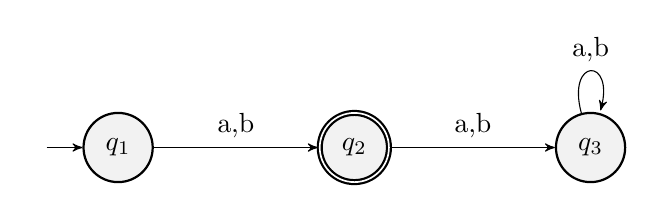
\begin{tikzpicture}
                \node[state, initial] (q1) {$q_1$};
                \node[state, right of=q1, accepting] (q2) {$q_2$};
                \node[state, right of=q2] (q3) {$q_3$};
                \draw
                    (q1) edge[above] node{a,b} (q2)
                    (q2) edge[above] node{a,b} (q3)
                    (q3) edge[loop above] node{a,b} (q3)
                    ;
                \end{tikzpicture}
        \end{figure}
        Then the complement of the machine $M$ is
        \begin{figure}[H]
            \centering
            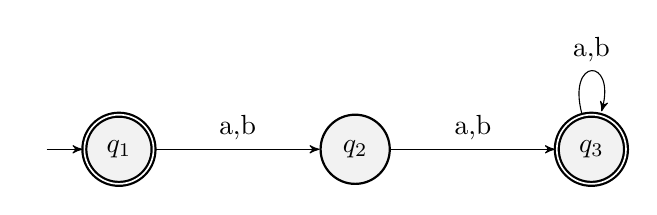
\begin{tikzpicture}
                \node[state, initial, accepting] (q1) {$q_1$};
                \node[state, right of=q1] (q2) {$q_2$};
                \node[state, right of=q2, accepting] (q3) {$q_3$};
                \draw
                    (q1) edge[above] node{a,b} (q2)
                    (q2) edge[above] node{a,b} (q3)
                    (q3) edge[loop above] node{a,b} (q3)
                    ;
                \end{tikzpicture}
        \end{figure}
    \end{itemize}
\end{proof}
\cleardoublepage
\begin{proof}{\textbf{1.6}}
\begin{itemize}
    \item [\textbf{a.}] Let $M$ be a machine that checks if
    the input string begins with a $1$ and ends with a $0$ then $M$
    is defined as
    \begin{figure}[H]
        \centering
        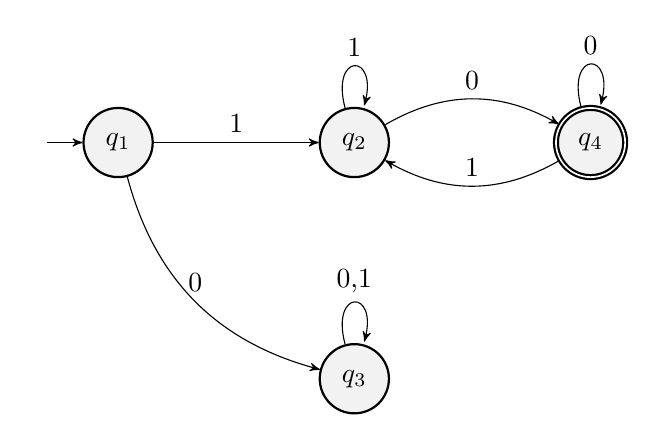
\begin{tikzpicture}
            \node[state, initial] (q1) {$q_1$};
            \node[state, right of=q1] (q2) {$q_2$};
            \node[state, below of=q2] (q3) {$q_3$};
            \node[state, right of=q2, accepting] (q4) {$q_4$};
            \draw
                (q1) edge[above] node{1} (q2)
                (q1) edge[above, bend right] node{0} (q3)
                (q2) edge[above, bend left] node{0} (q4)
                (q2) edge[loop above] node{1} (q2)
                (q3) edge[loop above] node{0,1} (q2)
                (q4) edge[above, bend left] node{1} (q2)
                (q4) edge[loop above] node{0} (q4)
                ;
            \end{tikzpicture}
    \end{figure}4
    \item [\textbf{b.}] Let $M$ be a machine that checks if
    the input string contains at least three $1$s then $M$
    is defined as
    \begin{figure}[H]
        \centering
        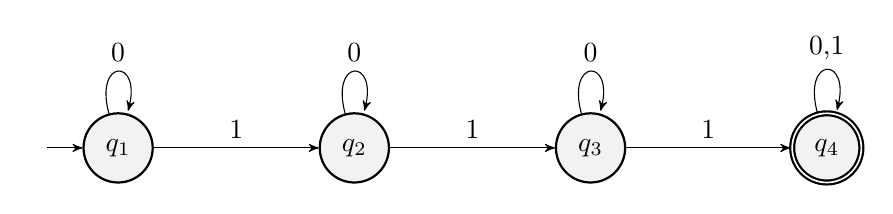
\begin{tikzpicture}
            \node[state, initial] (q1) {$q_1$};
            \node[state, right of=q1] (q2) {$q_2$};
            \node[state, right of=q2] (q3) {$q_3$};
            \node[state, right of=q3, accepting] (q4) {$q_4$};
            \draw
                (q1) edge[loop above] node{0} (q1)
                (q1) edge[above] node{1} (q2)
                (q2) edge[loop above] node{0} (q2)
                (q2) edge[above] node{1} (q3)
                (q3) edge[loop above] node{0} (q3)
                (q3) edge[above] node{1} (q4)
                (q4) edge[loop above] node{0,1} (q4)
                ;
            \end{tikzpicture}
    \end{figure}
    \item [\textbf{c.}] Let $M$ be a machine that checks if
    the input string contains the substring $0101$ then $M$
    is defined as
    \begin{figure}[H]
        \centering
        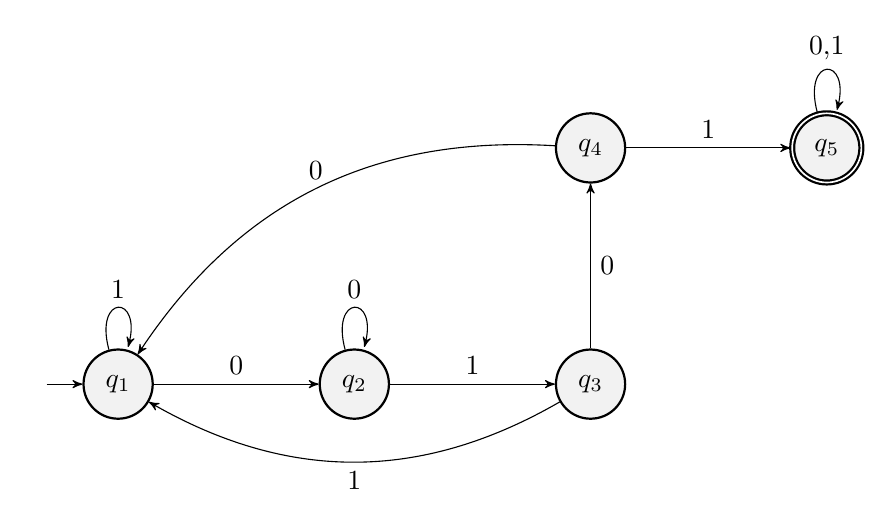
\begin{tikzpicture}
            \node[state, initial] (q1) {$q_1$};
            \node[state, right of=q1] (q2) {$q_2$};
            \node[state, right of=q2] (q3) {$q_3$};
            \node[state, above of=q3] (q4) {$q_4$};
            \node[state, right of=q4, accepting] (q5) {$q_5$};
            \draw
                (q1) edge[loop above] node{1} (q1)
                (q1) edge[above] node{0} (q2)
                (q2) edge[loop above] node{0} (q2)
                (q2) edge[above] node{1} (q3)
                (q3) edge[right] node{0} (q4)
                (q3) edge[below, bend left] node{1} (q1)
                (q4) edge[above, bend right] node{0} (q1)
                (q4) edge[above] node{1} (q5)
                (q5) edge[loop above] node{0,1} (q5)
                ;
            \end{tikzpicture}
    \end{figure}
\cleardoublepage
    \item[\textbf{d.}] Let $M$ be a machine that checks if
    the input string has length at least $3$ and its third symbol is a $0$
    then $M$ is defined as
    \begin{figure}[H]
        \centering
        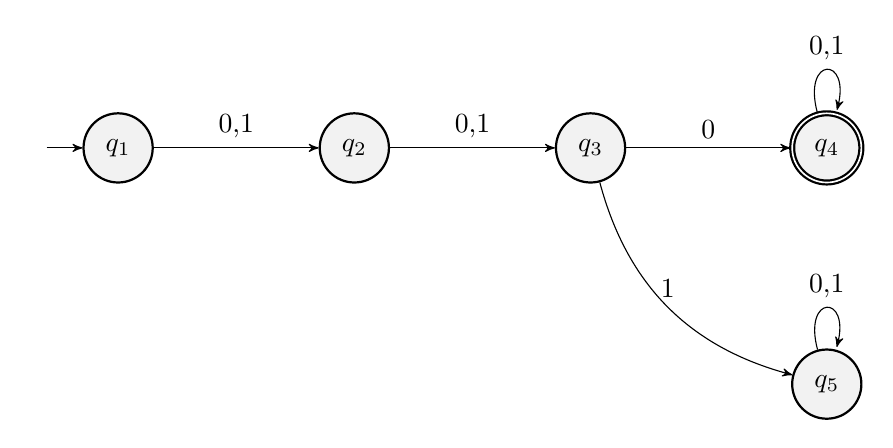
\begin{tikzpicture}
            \node[state, initial] (q1) {$q_1$};
            \node[state, right of=q1] (q2) {$q_2$};
            \node[state, right of=q2] (q3) {$q_3$};
            \node[state, right of=q3, accepting] (q4) {$q_4$};
            \node[state, below of=q4] (q5) {$q_5$};
            \draw
                (q1) edge[above] node{0,1} (q2)
                (q2) edge[above] node{0,1} (q3)
                (q3) edge[above] node{0} (q4)
                (q3) edge[above, bend right] node{1} (q5)
                (q4) edge[loop above] node{0,1} (q4)
                (q5) edge[loop above] node{0,1} (q5)
                ;
            \end{tikzpicture}
    \end{figure}
    \item[\textbf{e.}] Let $M$ be a machine that checks if
    the input string starts with $0$ and has odd length or starts with $1$
    and has even length then $M$ is defined as
    \begin{figure}[H]
        \centering
        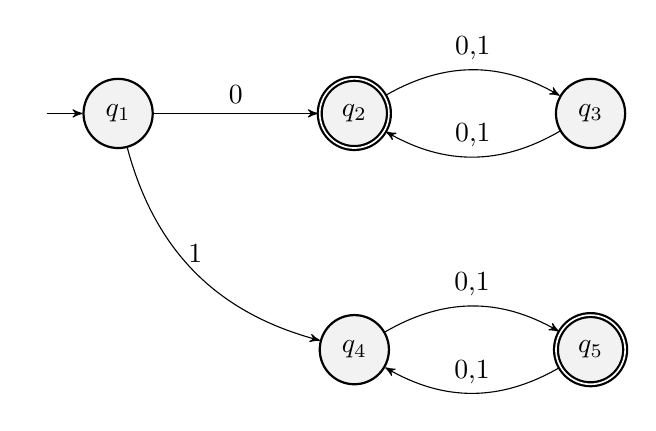
\begin{tikzpicture}
            \node[state, initial] (q1) {$q_1$};
            \node[state, right of=q1, accepting] (q2) {$q_2$};
            \node[state, right of=q2] (q3) {$q_3$};
            \node[state, below of=q2] (q4) {$q_4$};
            \node[state, right of=q4, accepting] (q5) {$q_5$};
            \draw
                (q1) edge[above] node{0} (q2)
                (q1) edge[above, bend right] node{1} (q4)
                (q2) edge[above, bend left] node{0,1} (q3)
                (q3) edge[above, bend left] node{0,1} (q2)
                (q4) edge[above, bend left] node{0,1} (q5)
                (q5) edge[above, bend left] node{0,1} (q4)
                ;
            \end{tikzpicture}
    \end{figure}
    \item[\textbf{f.}] Let $M$ be a machine that checks if
    the input string doesn't contain the substring $110$ then $M$ is defined as
    \begin{figure}[H]
        \centering
        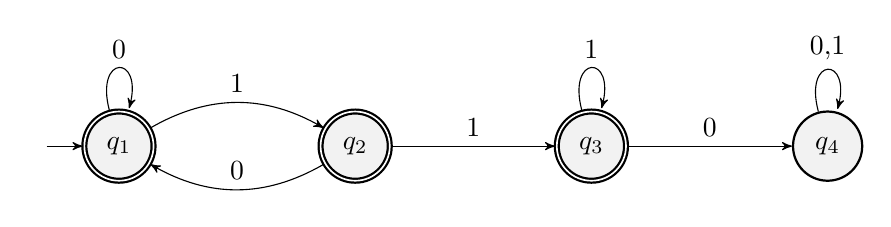
\begin{tikzpicture}
            \node[state, initial, accepting] (q1) {$q_1$};
            \node[state, right of=q1, accepting] (q2) {$q_2$};
            \node[state, right of=q2, accepting] (q3) {$q_3$};
            \node[state, right of=q3] (q4) {$q_4$};
            \draw
                (q1) edge[loop above] node{0} (q1)
                (q1) edge[above, bend left] node{1} (q2)
                (q2) edge[above, bend left] node{0} (q1)
                (q2) edge[above] node{1} (q3)
                (q3) edge[loop above] node{1} (q3)
                (q3) edge[above] node{0} (q4)
                (q4) edge[loop above] node{0,1} (q4)
                ;
            \end{tikzpicture}
    \end{figure}
\cleardoublepage
    \item[\textbf{g.}] Let $M$ be a machine that checks if
    the input string has a length at most $5$ then $M$ is defined as
    \begin{figure}[H]
        \centering
        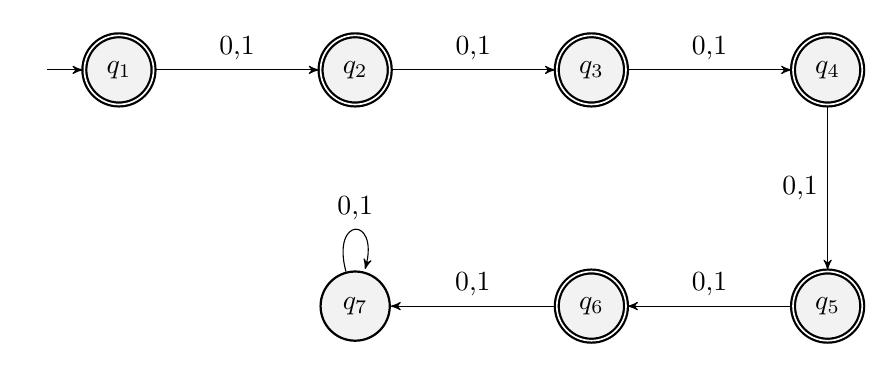
\begin{tikzpicture}
            \node[state, initial, accepting] (q1) {$q_1$};
            \node[state, right of=q1, accepting] (q2) {$q_2$};
            \node[state, right of=q2, accepting] (q3) {$q_3$};
            \node[state, right of=q3, accepting] (q4) {$q_4$};
            \node[state, below of=q4, accepting] (q5) {$q_5$};
            \node[state, left of=q5, accepting] (q6) {$q_6$};
            \node[state, left of=q6] (q7) {$q_7$};
            \draw
                (q1) edge[above] node{0,1} (q2)
                (q2) edge[above] node{0,1} (q3)
                (q3) edge[above] node{0,1} (q4)
                (q4) edge[left] node{0,1} (q5)
                (q5) edge[above] node{0,1} (q6)
                (q6) edge[above] node{0,1} (q7)
                (q7) edge[loop above] node{0,1} (q7)
                ;
            \end{tikzpicture}
    \end{figure}
    \item[\textbf{h.}] Let $M$ be a machine that checks if
    the input string is any string except 11 or 111 then $M$ is defined as
    \begin{figure}[H]
        \centering
        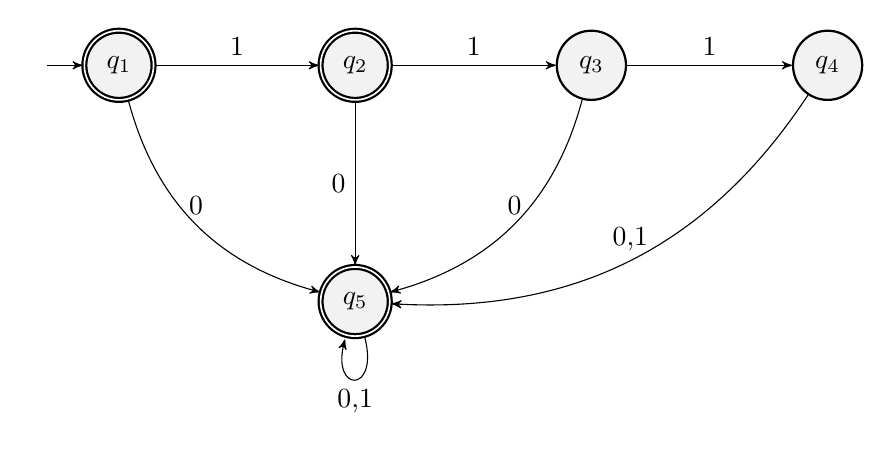
\begin{tikzpicture}
            \node[state, initial, accepting] (q1) {$q_1$};
            \node[state, right of=q1, accepting] (q2) {$q_2$};
            \node[state, right of=q2] (q3) {$q_3$};
            \node[state, right of=q3] (q4) {$q_4$};
            \node[state, below of=q2, accepting] (q5) {$q_5$};
            \draw
                (q1) edge[above] node{1} (q2)
                (q1) edge[above, bend right] node{0} (q5)
                (q2) edge[above] node{1} (q3)
                (q2) edge[left] node{0} (q5)
                (q3) edge[above] node{1} (q4)
                (q3) edge[above, bend left] node{0} (q5)
                (q4) edge[above,bend left] node{0,1} (q5)
                (q5) edge[loop below] node{0,1} (q5)
                ;
            \end{tikzpicture}
    \end{figure}
    \item[\textbf{i.}] Let $M$ be a machine that checks if
    the input string has a 1 in every odd position then $M$ is defined as
    \begin{figure}[H]
        \centering
        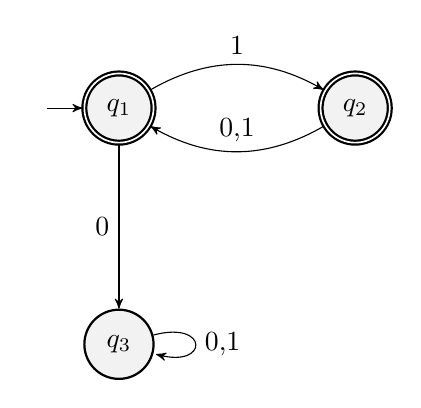
\begin{tikzpicture}
            \node[state, initial, accepting] (q1) {$q_1$};
            \node[state, right of=q1, accepting] (q2) {$q_2$};
            \node[state, below of=q1] (q3) {$q_3$};
            \draw
                (q1) edge[above, bend left] node{1} (q2)
                (q1) edge[left] node{0} (q3)
                (q2) edge[above, bend left] node{0,1} (q1)
                (q3) edge[loop right] node{0,1} (q3)
                ;
            \end{tikzpicture}
    \end{figure}
\cleardoublepage
    \item[\textbf{j.}] Let $M$ be a machine that checks if
    the input string has at least two 0s and at most one 1 then $M$ is defined
    as
    \begin{figure}[H]
        \centering
        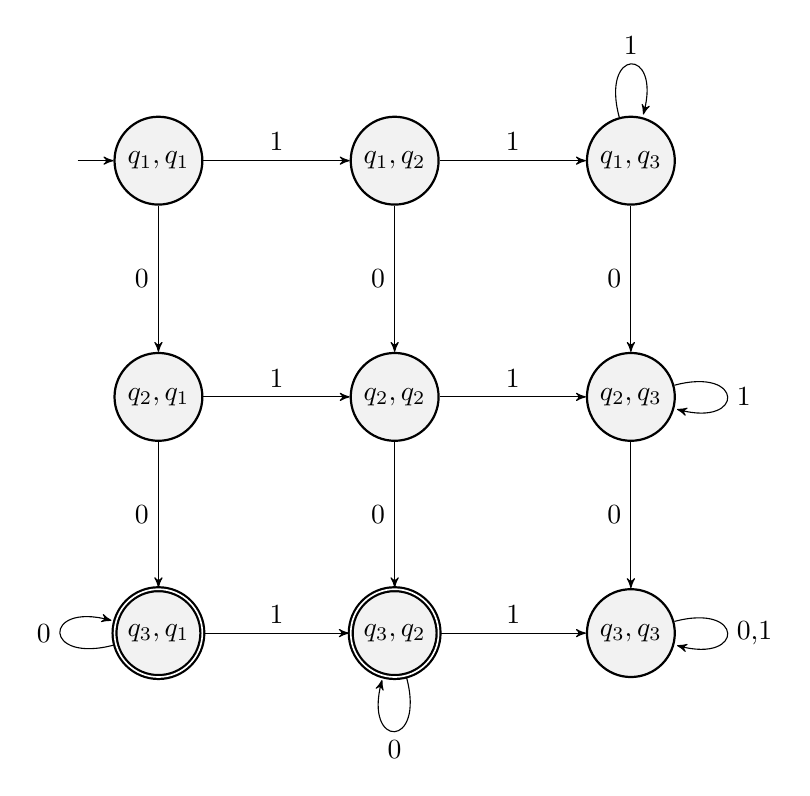
\begin{tikzpicture}
            \node[state, initial] (q1q1) {$q_1,q_1$};
            \node[state, right of=q1q1] (q1q2) {$q_1,q_2$};
            \node[state, right of=q1q2] (q1q3) {$q_1,q_3$};
            \node[state, below of=q1q1] (q2q1) {$q_2,q_1$};
            \node[state, right of=q2q1] (q2q2) {$q_2,q_2$};
            \node[state, right of=q2q2] (q2q3) {$q_2,q_3$};
            \node[state, below of=q2q1, accepting] (q3q1) {$q_3,q_1$};
            \node[state, right of=q3q1, accepting] (q3q2) {$q_3,q_2$};
            \node[state, right of=q3q2] (q3q3) {$q_3,q_3$};
            \draw
                (q1q1) edge[left] node{0} (q2q1)
                (q1q1) edge[above] node{1} (q1q2)
                (q1q2) edge[left] node{0} (q2q2)
                (q1q2) edge[above] node{1} (q1q3)
                (q1q3) edge[left] node{0} (q2q3)
                (q1q3) edge[loop above] node{1} (q1q3)

                (q2q1) edge[left] node{0} (q3q1)
                (q2q1) edge[above] node{1} (q2q2)
                (q2q2) edge[left] node{0} (q3q2)
                (q2q2) edge[above] node{1} (q2q3)
                (q2q3) edge[left] node{0} (q3q3)
                (q2q3) edge[loop right] node{1} (q2q3)

                (q3q1) edge[loop left] node{0} (q3q1)
                (q3q1) edge[above] node{1} (q3q2)
                (q3q2) edge[loop below] node{0} (q3q2)
                (q3q2) edge[above] node{1} (q3q3)
                (q3q3) edge[loop right] node{0,1} (q3q3)
                ;
            \end{tikzpicture}
    \end{figure}
    \item[\textbf{k.}] Let $M$ be a machine that checks if
    the input string is $\varepsilon$ or $0$ then $M$ is defined as
    \begin{figure}[H]
        \centering
        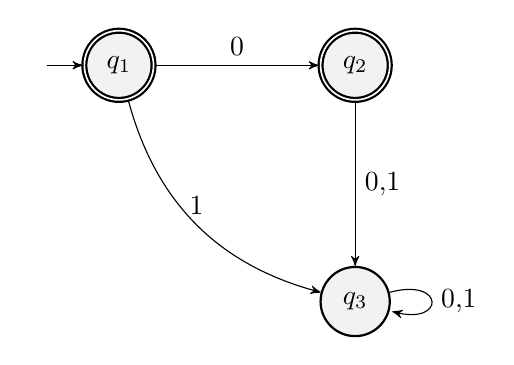
\begin{tikzpicture}
            \node[state, initial, accepting] (q1) {$q_1$};
            \node[state, right of=q1, accepting] (q2) {$q_2$};
            \node[state, below of=q2] (q3) {$q_3$};
            \draw
                (q1) edge[above] node{0} (q2)
                (q1) edge[above, bend right] node{1} (q3)
                (q2) edge[right] node{0,1} (q3)
                (q3) edge[loop right] node{0,1} (q3)
                ;
            \end{tikzpicture}
    \end{figure}
    \cleardoublepage
    \item[\textbf{l.}] Let $M$ be a machine that checks if
    the input string contains an even number of $0$s or exactly two 1s
    then $M$ is defined as
    \begin{figure}[H]
        \centering
        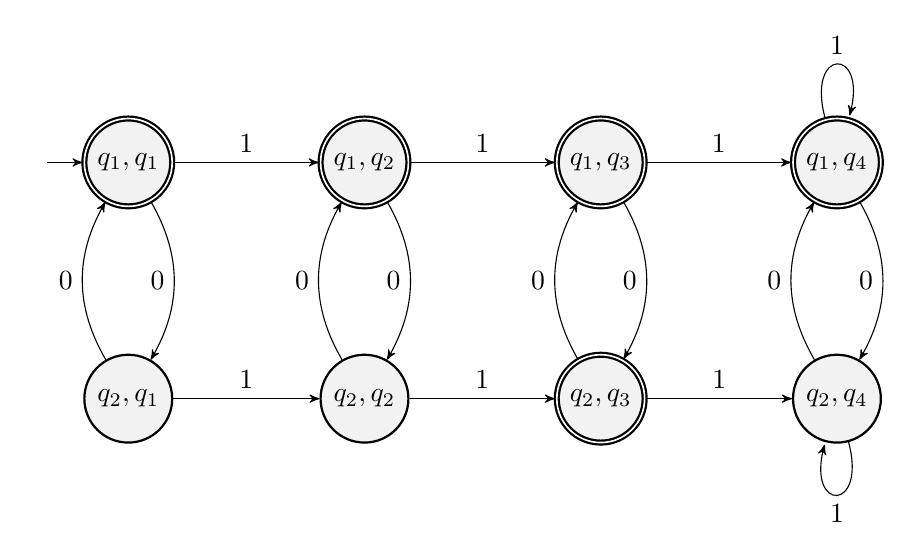
\begin{tikzpicture}
            \node[state, initial, accepting] (q1q1) {$q_1,q_1$};
            \node[state, right of=q1q1, accepting] (q1q2) {$q_1, q_2$};
            \node[state, right of=q1q2, accepting] (q1q3) {$q_1, q_3$};
            \node[state, right of=q1q3, accepting] (q1q4) {$q_1, q_4$};
            \node[state, below of=q1q1] (q2q1) {$q_2, q_1$};
            \node[state, right of=q2q1] (q2q2) {$q_2, q_2$};
            \node[state, right of=q2q2, accepting] (q2q3) {$q_2, q_3$};
            \node[state, right of=q2q3] (q2q4) {$q_2, q_4$};
            \draw
                (q1q1) edge[left, bend left] node{0} (q2q1)
                (q1q1) edge[above] node{1} (q1q2)
                (q1q2) edge[left, bend left] node{0} (q2q2)
                (q1q2) edge[above] node{1} (q1q3)
                (q1q3) edge[left, bend left] node{0} (q2q3)
                (q1q3) edge[above] node{1} (q1q4)
                (q1q4) edge[left, bend left] node{0} (q2q4)
                (q1q4) edge[loop above] node{1} (q1q4)

                (q2q1) edge[left, bend left] node{0} (q1q1)
                (q2q1) edge[above] node{1} (q2q2)
                (q2q2) edge[left, bend left] node{0} (q1q2)
                (q2q2) edge[above] node{1} (q2q3)
                (q2q3) edge[left, bend left] node{0} (q1q3)
                (q2q3) edge[above] node{1} (q2q4)
                (q2q4) edge[left, bend left] node{0} (q1q4)
                (q2q4) edge[loop below] node{1} (q2q4)
                ;
            \end{tikzpicture}
    \end{figure}
    \item[\textbf{m.}] Let $M$ be a machine that checks if
    the input string is the empty set then $M$ is defined as
    \begin{figure}[H]
        \centering
        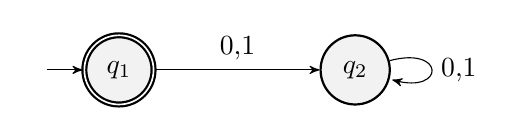
\begin{tikzpicture}
            \node[state, initial, accepting] (q1) {$q_1$};
            \node[state, right of=q1] (q2) {$q_2$};
            \draw
                (q1) edge[above] node{0,1} (q2)
                (q2) edge[loop right] node{0,1} (q2)
                ;
            \end{tikzpicture}
    \end{figure}
    \item[\textbf{n.}] Let $M$ be a machine that checks if
    the input string is any string except the empty set then $M$ is defined as
    \begin{figure}[H]
        \centering
        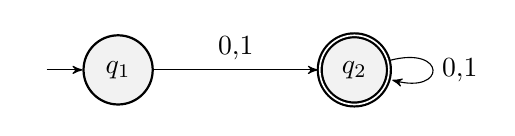
\begin{tikzpicture}
            \node[state, initial] (q1) {$q_1$};
            \node[state, right of=q1, accepting] (q2) {$q_2$};
            \draw
                (q1) edge[above] node{0,1} (q2)
                (q2) edge[loop right] node{0,1} (q2)
                ;
            \end{tikzpicture}
    \end{figure}
\end{itemize}
\end{proof}

\cleardoublepage
\begin{proof}{\textbf{1.7}}
    \begin{itemize}
        \item [\textbf{a.}] Let $M$ be the NFA that recognizes the language
        $\{w : w\text{ ends with }00\}$ with only three states
        \begin{figure}[H]
            \centering
            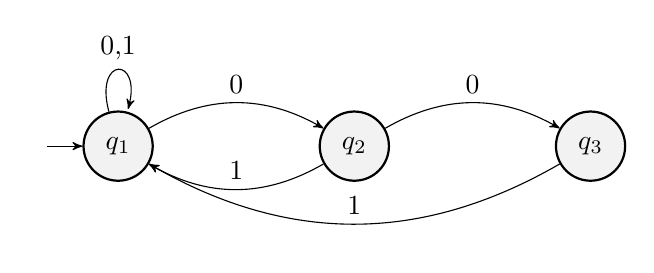
\begin{tikzpicture}
                \node[state, initial] (q1) {$q_1$};
                \node[state, right of=q1] (q2) {$q_2$};
                \node[state, right of=q2] (q3) {$q_3$};
                \draw
                    (q1) edge[loop above] node{0,1} (q1)
                    (q1) edge[above, bend left] node{0} (q2)
                    (q2) edge[above, bend left] node{1} (q1)
                    (q2) edge[above, bend left] node{0} (q3)
                    (q3) edge[above, bend left] node{1} (q1)
                    ;
                \end{tikzpicture}
        \end{figure}
        \item [\textbf{b.}] Let $M$ be the NFA that recognizes the strings
        that have the substring $0101$ then $M$ is defined as
        \begin{figure}[H]
            \centering
            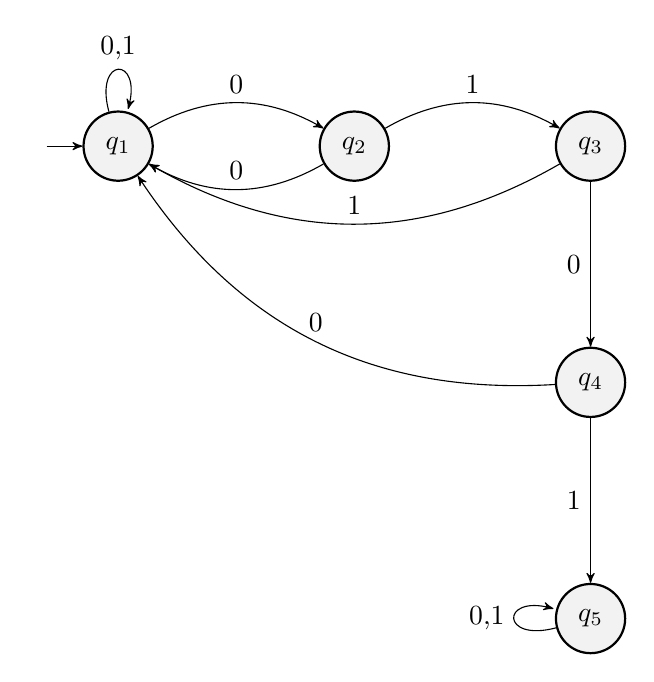
\begin{tikzpicture}
                \node[state, initial] (q1) {$q_1$};
                \node[state, right of=q1] (q2) {$q_2$};
                \node[state, right of=q2] (q3) {$q_3$};
                \node[state, below of=q3] (q4) {$q_4$};
                \node[state, below of=q4] (q5) {$q_5$};
                \draw
                    (q1) edge[loop above] node{0,1} (q1)
                    (q1) edge[above, bend left] node{0} (q2)
                    (q2) edge[above, bend left] node{0} (q1)
                    (q2) edge[above, bend left] node{1} (q3)
                    (q3) edge[above, bend left] node{1} (q1)
                    (q3) edge[left] node{0} (q4)
                    (q4) edge[above, bend left] node{0} (q1)
                    (q4) edge[left] node{1} (q5)
                    (q5) edge[loop left] node{0,1} (q5)
                    ;
                \end{tikzpicture}
        \end{figure}
        \cleardoublepage
        \item [\textbf{c.}] Let $M$ be the NFA that recognizes the strings
        that have an even number of 0s or exactly two 1s then $M$ is defined as
        \begin{figure}[H]
            \centering
            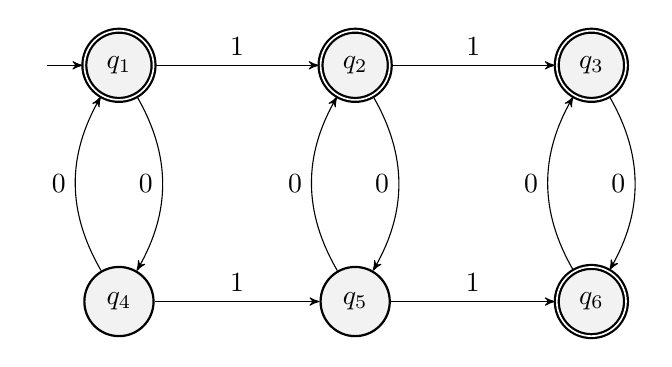
\begin{tikzpicture}
                \node[state, initial, accepting] (q1) {$q_1$};
                \node[state, right of=q1, accepting] (q2) {$q_2$};
                \node[state, right of=q2, accepting] (q3) {$q_3$};
                \node[state, below of=q1] (q4) {$q_4$};
                \node[state, right of=q4] (q5) {$q_5$};
                \node[state, right of=q5, accepting] (q6) {$q_6$};
                \draw
                    (q1) edge[left, bend left] node{0} (q4)
                    (q1) edge[above] node{1} (q2)
                    (q2) edge[left, bend left] node{0} (q5)
                    (q2) edge[above] node{1} (q3)
                    (q3) edge[left, bend left] node{0} (q6)
    
                    (q4) edge[left, bend left] node{0} (q1)
                    (q4) edge[above] node{1} (q5)
                    (q5) edge[left, bend left] node{0} (q2)
                    (q5) edge[above] node{1} (q6)
                    (q6) edge[left, bend left] node{0} (q3)
                    ;
                \end{tikzpicture}
        \end{figure}
        \item [\textbf{d.}] Let $M$ be the NFA that recognizes the string
        0 then $M$ is defined as
        \begin{figure}[H]
            \centering
            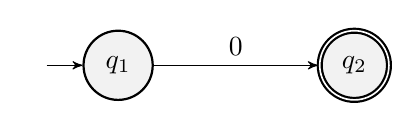
\begin{tikzpicture}
                \node[state, initial] (q1) {$q_1$};
                \node[state, right of=q1, accepting] (q2) {$q_2$};
                \draw
                    (q1) edge[above] node{0} (q2)
                    ;
                \end{tikzpicture}
        \end{figure}

        \item [\textbf{e.}] Let $M$ be the NFA that recognizes the strings
        of the form $0^*1^*0^+$ then $M$ is defined as
        \begin{figure}[H]
            \centering
            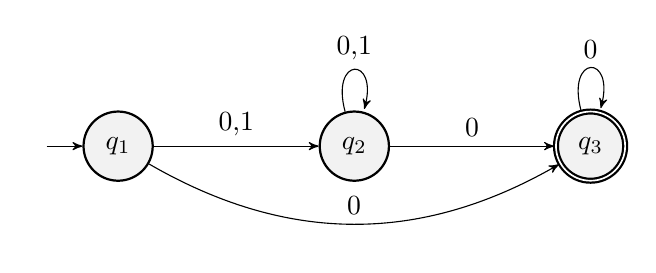
\begin{tikzpicture}
                \node[state, initial] (q1) {$q_1$};
                \node[state, right of=q1] (q2) {$q_2$};
                \node[state, right of=q2, accepting] (q3) {$q_3$};
                \draw
                    (q1) edge[above] node{0,1} (q2)
                    (q1) edge[above, bend right] node{0} (q3)
                    (q2) edge[loop above] node{0,1} (q2)
                    (q2) edge[above] node{0} (q3)
                    (q3) edge[loop above] node{0} (q3)
                    ;
            \end{tikzpicture}
        \end{figure}

        \item [\textbf{f.}] Let $M$ be the NFA that recognizes the strings
        of the form $1^*(001^+)^*$ then $M$ is defined as
        \begin{figure}[H]
            \centering
            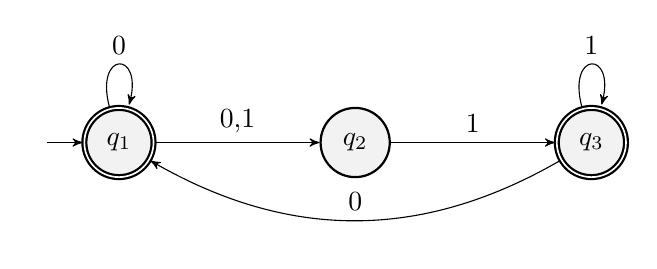
\begin{tikzpicture}
                \node[state, initial, accepting] (q1) {$q_1$};
                \node[state, right of=q1] (q2) {$q_2$};
                \node[state, right of=q2, accepting] (q3) {$q_3$};
                \draw
                    (q1) edge[loop above] node{0} (q1)
                    (q1) edge[above] node{0,1} (q2)
                    (q2) edge[above] node{1} (q3)
                    (q3) edge[loop above] node{1} (q3)
                    (q3) edge[above, bend left] node{0} (q1)
                    ;
            \end{tikzpicture}
        \end{figure}

        \item [\textbf{g.}] Let $M$ be the NFA that recognizes the language
        $\{\varepsilon\}$ then $M$ is defined as
        \begin{figure}[H]
            \centering
            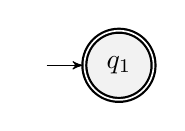
\begin{tikzpicture}
                \node[state, initial, accepting] (q1) {$q_1$};
                \draw
                    ;
            \end{tikzpicture}
        \end{figure}
\cleardoublepage
        \item [\textbf{h.}] Let $M$ be the NFA that recognizes the language
        $0^*$ then $M$ is defined as
        \begin{figure}[H]
            \centering
            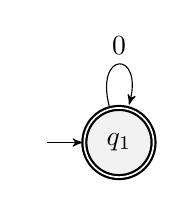
\begin{tikzpicture}
                \node[state, initial, accepting] (q1) {$q_1$};
                \draw
                    (q1) edge[loop above] node{0} (q1)
                    ;
            \end{tikzpicture}
        \end{figure}

    \end{itemize}
\end{proof}

\begin{proof}{\textbf{1.8}}
\begin{itemize}
    \item [\textbf{a.}] Let $M$ be a machine that recognizes both languages
    described in Exercises 1.6a and 1.6b then
    \begin{figure}[H]
        \centering
        \begin{tikzpicture}
            \node[state, initial] (q0) {$q_0$};
            \node[state, above of=q0] (q1) {$q_1$};
            \node[state, right of=q1] (q2) {$q_2$};
            \node[state, above of=q2] (q3) {$q_3$};
            \node[state, right of=q2, accepting] (q4) {$q_4$};
            
            \node[state, below of=q0] (q5) {$q_5$};
            \node[state, right of=q5] (q6) {$q_6$};
            \node[state, right of=q6] (q7) {$q_7$};
            \node[state, right of=q7, accepting] (q8) {$q_8$};
            \draw
                (q0) edge[left] node{$\varepsilon$} (q1)
                (q0) edge[left] node{$\varepsilon$} (q5)

                (q1) edge[above] node{1} (q2)
                (q1) edge[below, bend left] node{0} (q3)
                (q2) edge[above, bend left] node{0} (q4)
                (q2) edge[loop above] node{1} (q2)
                (q3) edge[loop above] node{0,1} (q2)
                (q4) edge[above, bend left] node{1} (q2)
                (q4) edge[loop above] node{0} (q4)

                (q5) edge[loop below] node{0} (q5)
                (q5) edge[above] node{1} (q6)
                (q6) edge[loop below] node{0} (q6)
                (q6) edge[above] node{1} (q7)
                (q7) edge[loop below] node{0} (q7)
                (q7) edge[above] node{1} (q8)
                (q8) edge[loop below] node{0,1} (q8)
            ;
            \end{tikzpicture}
        \end{figure}
\end{itemize}
\end{proof}
\cleardoublepage
\begin{proof}{\textbf{1.9}}
    \begin{itemize}
        \item [\textbf{a.}] Let $M$ be a machine that recognizes the
        concatenation of the languages  described in Exercises 1.6g and 1.6i
        then
        \begin{figure}[H]
            \centering
            \begin{tikzpicture}
                \node[state, initial] (q1) {$q_1$};
                \node[state, below of=q1] (q2) {$q_2$};
                \node[state, below of=q2] (q3) {$q_3$};
                \node[state, below of=q3] (q4) {$q_4$};
                \node[state, right of=q4] (q5) {$q_5$};
                \node[state, right of=q5] (q6) {$q_6$};
                \node[state, right of=q6] (q7) {$q_7$};
                \node[state, right of=q1, accepting] (q8) {$q_8$};
                \node[state, right of=q8, accepting] (q9) {$q_9$};
                \node[state, above of=q8] (q10) {$q_{10}$};

                \draw
                    (q1) edge[left] node{0,1} (q2)
                    (q2) edge[left] node{0,1} (q3)
                    (q3) edge[left] node{0,1} (q4)
                    (q4) edge[above] node{0,1} (q5)
                    (q5) edge[above] node{0,1} (q6)
                    (q6) edge[above] node{0,1} (q7)
                    (q7) edge[loop above] node{0,1} (q7)
                    (q1) edge[above] node{$\epsilon$} (q8)
                    (q2) edge[above] node{$\epsilon$} (q8)
                    (q3) edge[left] node{$\epsilon$} (q8)
                    (q4) edge[left] node{$\epsilon$} (q8)
                    (q5) edge[left] node{$\epsilon$} (q8)
                    (q6) edge[left] node{$\epsilon$} (q8)

                    (q8) edge[above, bend left] node{1} (q9)
                    (q8) edge[right] node{0} (q10)
                    (q9) edge[above, bend left] node{0,1} (q8)
                    (q10) edge[loop right] node{0,1} (q10)
                    ;
                \end{tikzpicture}
        \end{figure}
    \end{itemize}
\end{proof}
\cleardoublepage
\begin{proof}{\textbf{1.10}}
\begin{itemize}
    \item [\textbf{a.}]
    Let $M$ be a machine that recognizes the star of the language described in
    Exercise 1.6b then
    \begin{figure}[H]
        \centering
        \begin{tikzpicture}
            \node[state, initial, accepting] (q0) {$q_0$};
            \node[state, below of=q0] (q1) {$q_1$};
            \node[state, right of=q1] (q2) {$q_2$};
            \node[state, right of=q2] (q3) {$q_3$};
            \node[state, right of=q3, accepting] (q4) {$q_4$};
            \draw
                (q0) edge[right] node{$\epsilon$} (q1)
                (q1) edge[loop left] node{0} (q1)
                (q1) edge[above] node{1} (q2)
                (q2) edge[loop above] node{0} (q2)
                (q2) edge[above] node{1} (q3)
                (q3) edge[loop above] node{0} (q3)
                (q3) edge[above] node{1} (q4)
                (q4) edge[loop right] node{0,1} (q4)
                (q4) edge[above, bend right] node{$\epsilon$} (q0)
                ;
            \end{tikzpicture}
    \end{figure}
\end{itemize}
\end{proof}
\begin{proof}{\textbf{1.11}}
    Given that every NFA has an equivalent DFA, and we can convert a DFA into
    a GNFA by adding an $\epsilon$ arrow from every accept state to one
    accept state, then we can convert every NFA to an equivalent one that has
    a single accept state.  
\end{proof}
\cleardoublepage
\begin{proof}{\textbf{1.12}}
    Let
    \begin{align*}
        D = &\{w | w \text{ contains an even number of a's and an odd number}\\
        &\text{of b's and does not contain the substring } ab\}
    \end{align*}
    Then we can write the regular expression that generates $D$ as follows
    \begin{align*}
        (bb)^*b(aa)^*
    \end{align*}
    Finally, the DFA that recognizes $D$ is given by
    \begin{figure}[H]
        \centering
        \begin{tikzpicture}
            \node[state, initial] (q0) {$q_0$};
            \node[state, right of=q0, accepting] (q1) {$q_1$};
            \node[state, right of=q1] (q2) {$q_2$};
            \node[state, above of=q1] (q3) {$q_3$};
            \node[state, above of=q3] (q4) {$q_4$};
            \draw
                (q0) edge[above] node{b} (q1)
                (q0) edge[bend left, left] node{a} (q4)
                (q1) edge[bend left, above] node{b} (q2)
                (q1) edge[bend right, left] node{a} (q3)
                (q2) edge[bend left, above] node{b} (q1)
                (q2) edge[bend right, right] node{a} (q4)
                (q3) edge[bend right, left] node{a} (q1)
                (q3) edge[right] node{b} (q4)
                (q4) edge[loop above] node{a,b} (q4)
                ;
            \end{tikzpicture}
    \end{figure}
\end{proof}
\cleardoublepage
\begin{proof}{\textbf{1.13}}
    Let $\overline{F}$ be the language that recognizes all strings that 
    contain a pair of $1$s separated by an odd number of $0$s then the NFA
    with four states for this language is given by
    \begin{figure}[H]
        \centering
        \begin{tikzpicture}
            \node[state, initial] (q0) {$q_0$};
            \node[state, right of=q0] (q1) {$q_1$};
            \node[state, right of=q1] (q2) {$q_2$};
            \node[state, right of=q2, accepting] (q3) {$q_3$};
            \draw
                (q0) edge[above] node{1} (q1)
                (q1) edge[bend left, above] node{0} (q2)
                (q2) edge[bend left, above] node{0} (q1)
                (q2) edge[above] node{1} (q3)
                ;
            \end{tikzpicture}
    \end{figure}
    Then $F$ the complement of $\overline{F}$ is the language that recognizes
    strings that do not contain a pair of $1$s that are separated by an odd
    number of symbols. A DFA for this language is shown below
    \begin{figure}[H]
        \centering
        \begin{tikzpicture}
            \node[state, initial, accepting] (q0) {$q_0$};
            \node[state, right of=q0, accepting] (q1) {$q_1$};
            \node[state, right of=q1,accepting] (q2) {$q_2$};
            \node[state, right of=q2] (q3) {$q_3$};
            % \node[state, below of=q1] (q4) {$q_4$};
            \draw
                (q0) edge[above] node{1} (q1)
                (q0) edge[loop above] node{0} (q0)
                (q1) edge[bend left, above] node{0} (q2)
                (q1) edge[loop above] node{1} (q1)
                (q2) edge[bend left, above] node{0} (q1)
                (q2) edge[above] node{1} (q3)
                (q3) edge[loop above] node{1, 0} (q3)
                ;
            \end{tikzpicture}
    \end{figure}
\end{proof}
\cleardoublepage
\begin{proof}{\textbf{1.14}}
\begin{itemize}
    \item [\textbf{a.}] If $M$ is a DFA that recognizes the language $B$, then
    there are finitely many states that are accept states and hence the rest
    are non-accept states. Taking the non-accept states as accept states for 
    a new DFA $M'$ we would accept all the strings that $M$ doesn't
    accept. Hence $M'$ recognizes the complement of $B$ i.e. $\overline{B}$.
    Therefore given that there is always a DFA $M'$ that accepts
    $\overline{B}$ then the class of regular languages is closed under
    complement.
    \item [\textbf{b.}] Let $M$ be an NFA that recognizes the language
    $C$ described by the regular expression $1^+$ over $\{0,1\}$ then $M$
    is given by
    \begin{figure}[H]
        \centering
        \begin{tikzpicture}
            \node[state, initial] (q0) {$q_0$};
            \node[state, right of=q0, accepting] (q1) {$q_1$};
            \draw
                (q0) edge[above] node{1} (q1)
                (q1) edge[loop above] node{1} (q1)
                ;
            \end{tikzpicture}
    \end{figure}
    Swapping the accept and nonaccept states in $M$ gives us 
    \begin{figure}[H]
        \centering
        \begin{tikzpicture}
            \node[state, initial, accepting] (q0) {$q_0$};
            \node[state, right of=q0] (q1) {$q_1$};
            \draw
                (q0) edge[above] node{1} (q1)
                (q1) edge[loop above] node{1} (q1)
                ;
            \end{tikzpicture}
    \end{figure}
    But this NFA accepts only the empty string $\epsilon$ which is not the
    complement of $C$ over $\{0,1\}$.

    If a language $A$ is recognized by an NFA then it's also recognized
    by a DFA, since there is always a DFA equivalent to the NFA then the 
    the language $A$ is closed under complement. This implies that the class
    of languages recognized by NFAs is closed under complement.

    But from the example we see that they are not always obtained by swapping
    the accept and non-accept states.
    \end{itemize}    
\end{proof}
\cleardoublepage
\begin{proof}{\textbf{1.16}}
Following the construction given in Theorem 1.39 we transform the given
NFAs into the following DFAs
\begin{itemize}
    \item [(a)] The first one give us 
    \begin{figure}[H]
        \centering
        \begin{tikzpicture}
            \node[state, initial, accepting] (1) {$\{1\}$};
            \node[state, right of=1] (2) {$\{2\}$};
            \node[state, below of=2] (e) {$\{\emptyset\}$};
            \node[state, below of=1, accepting] (12) {$\{1, 2\}$};
            \draw
                (1) edge[left] node{a} (12)
                (1) edge[above, bend left] node{b} (2)
                (2) edge[left] node{a} (e)
                (2) edge[above, bend left] node{b} (1)
                (12) edge[loop left] node{a,b} (12)
                (e) edge[loop left] node{a,b} (e)
                ;
            \end{tikzpicture}
    \end{figure}
    \item [\textbf{b.}] For this DFA we need $2^3 = 8$ states, hence
    \begin{figure}[H]
        \centering
        \begin{tikzpicture}
            \node[state] (e) {$\{\emptyset\}$};
            \node[state, right of=e, initial above] (1) {$\{1\}$};
            \node[state, below of=1, accepting] (2) {$\{2\}$};
            \node[state, right of=1] (3) {$\{3\}$};
            \node[state, below of=e, initial, accepting] (12) {$\{1,2\}$};
            \node[state, below of=2, accepting] (23) {$\{2,3\}$};
            \node[state, right of=23] (13) {$\{1,3\}$};
            \node[state, left of=23, accepting] (123) {$\{1,2,3\}$};
            \draw
                (e) edge[loop left] node{a,b} (e)
                (1) edge[above] node{a} (3)
                (1) edge[above] node{b} (e)
                (2) edge[above] node{a} (12)
                (2) edge[above] node{b} (e)
                (3) edge[above] node{a} (2)
                (3) edge[left] node{b} (23)
                (12) edge[left] node{a} (123)
                (12) edge[left] node{b} (e)
                (23) edge[above] node{a} (12)
                (23) edge[loop above] node{b} (23)
                (13) edge[above] node{a,b} (23)
                (123) edge[loop left] node{a} (123)
                (123) edge[above] node{b} (23)
                ;
            \end{tikzpicture}
    \end{figure}
\end{itemize}
\end{proof}
\cleardoublepage
\begin{proof}{\textbf{1.17}}
\begin{itemize}
\item [(a)] The NFA that recognizes the language $(01 \cup 001 \cup 010)^*$ is
\begin{figure}[H]
    \centering
    \begin{tikzpicture}
        \node[state, initial, accepting] (q1) {$q_1$};
        \node[state, right of=q1] (q2) {$q_2$};
        \node[state, right of=q2, accepting] (q3) {$q_3$};
        \node[state, below of=q3] (q4) {$q_4$};
        \draw
            (q1) edge[above] node{0} (q2)
            (q2) edge[above] node{0} (q4)
            (q2) edge[above, bend right] node{1} (q3)
            (q3) edge[above, bend right] node{0} (q2)
            (q3) edge[loop above] node{0} (q3)
            (q4) edge[right] node{1} (q3)
            ;
        \end{tikzpicture}
\end{figure}
\item [(b)] The equivalent DFA is then
\begin{figure}[H]
    \centering
    \begin{tikzpicture}
        \node[state, initial, accepting] (q1) {$\{q_1\}$};
        \node[state, right of=q1] (q4) {$\{q_4\}$};
        \node[state, right of=q4] (q2) {$\{q_2\}$};
        \node[state, above of=q4] (e) {$\{\emptyset\}$};
        \node[state, above of=q2, accepting] (q3) {$\{q_3\}$};
        % \node[state, below of=q2] (q1q2) {$\{q_1,q_2\}$};
        \node[state, right of=q3, accepting] (q2q3) {$\{q_2,q_3\}$};
        % \node[state, below of=e] (q1q3) {$\{q_1,q_3\}$};
        % \node[state, below of=q1] (q1q4) {$\{q_1,q_4\}$};
        % \node[state, below of=q1q2] (q2q4) {$\{q_2,q_4\}$};
        % \node[state, below of=q2q3] (q3q4) {$\{q_3,q_4\}$};
        % \node[state, below of=q1q3] (q1q2q3) {$\{q_1,q_2,q_3\}$};
        \node[state, right of=q2, accepting] (q2q3q4) {$\{q_2,q_3,q_4\}$};
        % \node[state, below of=q2q4] (q3q4q1) {$\{q_3,q_4,q_1\}$};
        % \node[state, below of=q3q4] (q1q2q4) {$\{q_1,q_2,q_4\}$};
        % \node[state, below of=q1q2q3] (q1q2q3q4) {$\{q_1,q_2,q_3,q4\}$};
        \draw
            (q1) edge[below, bend right] node{0} (q2)
            (q1) edge[above, bend left] node{1} (e)
            (q2) edge[above] node{0} (q4)
            (q2) edge[left] node{1} (q3)
            (q3) edge[above, bend left] node{0} (q2q3)
            (q3) edge[above] node{1} (e)
            (q4) edge[left] node{0} (e)
            (q4) edge[above] node{1} (q3)
            % (q1q2) edge[above] node{0} (q2q4)
            % (q1q2) edge[above] node{1} (q3)
            (q2q3) edge[right] node{0} (q2q3q4)
            (q2q3) edge[above, bend left] node{1} (q3)
            % (q1q3) edge[left] node{0} (q1q2q3)
            % (q1q3) edge[left] node{1} (e)
            % (q1q4) edge[above] node{0} (q2)
            % (q1q4) edge[above] node{1} (q3)
            % (q2q4) edge[above] node{0} (q4)
            % (q2q4) edge[above] node{1} (q3q4)
            % (q3q4) edge[above] node{0} (q2q3)
            % (q3q4) edge[above] node{1} (q3)
            % (q1q2q3) edge[above] node{0} (q2q3q4)
            % (q1q2q3) edge[above] node{1} (q3)
            (q2q3q4) edge[loop right] node{0} (q2q3q4)
            (q2q3q4) edge[above] node{1} (q3)
            % (q3q4q1) edge[above] node{0} (q2q3)
            % (q3q4q1) edge[above] node{1} (q3)
            % (q1q2q4) edge[above] node{0} (q2q4)
            % (q1q2q4) edge[above] node{1} (q3)
            % (q1q2q3q4) edge[above] node{0} (q2q3q4)
            % (q1q2q3q4) edge[above] node{1} (q3)
            ;
        \end{tikzpicture}
\end{figure}
\end{itemize}
\end{proof}
\cleardoublepage
\begin{proof}{\textbf{1.18}}
\begin{itemize}
    \item [a.] The regular expression generating the language
    \begin{align*}
        \{w | w\text{ begins with a 1 and ends with a 0}\}
    \end{align*}
    is 
    \begin{align*}
        1(0 \cup 1)^*0
    \end{align*}
    \item [b.] The regular expression generating the language
    \begin{align*}
        \{w | w\text{ contains at least three 1s}\}
    \end{align*}
    is 
    \begin{align*}
        0^*10^*10^*1(0 \cup 1)^*
    \end{align*}
\end{itemize}
\end{proof}
\cleardoublepage
\begin{proof}{\textbf{1.19}}
\begin{itemize}
    \item [a.] The NFA recognizing the regular expression
    $(0\cup 1)^*000(0\cup 1)^*$ is given by
    \begin{figure}[H]
        \centering
        \begin{tikzpicture}
            \node[state, initial] (q1) {$q_1$};
            \node[state, right of=q1] (q2) {$q_2$};
            \node[state, right of=q2] (q3) {$q_3$};
            \node[state, right of=q3, accepting] (q4) {$q_4$};
            \draw
                (q1) edge[loop above] node{0,1} (q1)
                (q1) edge[above] node{0} (q2)
                (q2) edge[above] node{0} (q3)
                (q3) edge[above] node{0} (q4)
                (q4) edge[loop above] node{0,1} (q4)
                ;
            \end{tikzpicture}
    \end{figure}
    \item [b.] The NFA recognizing the regular expression
    $(00)^*(11)$ is given by
    \begin{figure}[H]
        \centering
        \begin{tikzpicture}
            \node[state, initial] (q1) {$q_1$};
            \node[state, above of=q1] (q2) {$q_2$};
            \node[state, right of=q1] (q3) {$q_3$};
            \node[state, right of=q3, accepting] (q4) {$q_4$};
            \draw
                (q1) edge[bend right, right] node{0} (q2)
                (q1) edge[above] node{1} (q3)
                (q2) edge[bend right, left] node{0} (q1)
                (q3) edge[above] node{1} (q4)
                ;
            \end{tikzpicture}
    \end{figure}
    And the NFA recognizing the regular expression $01$ is 
    \begin{figure}[H]
        \centering
        \begin{tikzpicture}
            \node[state, initial] (q5) {$q_5$};
            \node[state, right of=q5] (q6) {$q_6$};
            \node[state, right of=q6, accepting] (q7) {$q_7$};
            \draw
                (q5) edge[above] node{0} (q6)
                (q6) edge[above] node{1} (q7)
                ;
            \end{tikzpicture}
    \end{figure}
    Given that regular languages are closed under union operation we can
    build an NFA that recognizes the regular expression $((00)^*(11)) \cup 01$
    as follows
    \begin{figure}[H]
        \centering
        \begin{tikzpicture}
            \node[state, initial] (q8) {$q_8$};
            \node[state, right of=q8] (q1) {$q_1$};
            \node[state, above of=q1] (q2) {$q_2$};
            \node[state, right of=q1] (q3) {$q_3$};
            \node[state, right of=q3, accepting] (q4) {$q_4$};
            \node[state, below of=q1] (q5) {$q_5$};
            \node[state, right of=q5] (q6) {$q_6$};
            \node[state, right of=q6, accepting] (q7) {$q_7$};
            \draw
                (q8) edge[above] node{$\varepsilon$} (q1)
                (q8) edge[above] node{$\varepsilon$} (q5)
                (q1) edge[bend right, right] node{0} (q2)
                (q1) edge[above] node{1} (q3)
                (q2) edge[bend right, left] node{0} (q1)
                (q3) edge[above] node{1} (q4)
                (q5) edge[above] node{0} (q6)
                (q6) edge[above] node{1} (q7)
                ;
            \end{tikzpicture}
    \end{figure}
    Finally, given that regular languages are closed under star operation we
    can build an NFA that recognizes the regular expression
    $$(((00)^*(11)) \cup 01)^*$$
    as follows
    \begin{figure}[H]
        \centering
        \begin{tikzpicture}
            \node[state, initial, accepting] (q0) {$q_0$};
            \node[state, below of=q0] (q8) {$q_8$};
            \node[state, above right of=q8] (q1) {$q_1$};
            \node[state, above of=q1] (q2) {$q_2$};
            \node[state, right of=q1] (q3) {$q_3$};
            \node[state, right of=q3, accepting] (q4) {$q_4$};
            \node[state, below right of=q8] (q5) {$q_5$};
            \node[state, right of=q5] (q6) {$q_6$};
            \node[state, right of=q6, accepting] (q7) {$q_7$};
            \draw
                (q0) edge[left] node{$\varepsilon$} (q8)
                (q8) edge[above] node{$\varepsilon$} (q1)
                (q8) edge[above] node{$\varepsilon$} (q5)
                (q1) edge[bend right, right] node{0} (q2)
                (q1) edge[above] node{1} (q3)
                (q2) edge[bend right, left] node{0} (q1)
                (q3) edge[above] node{1} (q4)
                (q5) edge[below] node{0} (q6)
                (q6) edge[below] node{1} (q7)
                (q4) edge[above] node{$\varepsilon$} (q8)
                (q7) edge[above] node{$\varepsilon$} (q8)
                ;
            \end{tikzpicture}
    \end{figure}
    \item [c.] The NFA recognizing the regular expression $\emptyset^*$
    is given by
    \begin{figure}[H]
        \centering
        \begin{tikzpicture}
            \node[state, initial, accepting] (q1) {$q_1$};
            \draw ;
            \end{tikzpicture}
    \end{figure}
\end{itemize}
\end{proof}
\cleardoublepage
\begin{proof}{\textbf{1.20}}
\begin{itemize}
    \item [a.] $a^*b^*$:\\
    Member strings are $a$ and $b$ and not member strings are $aba$ and $ba$.
    \item [b.] $a(ba)^*b$:\\
    Member strings are $ab$ and $abab$ and not member strings are $abb$ and $aa$.
    \item [g.] $(\varepsilon \cup a)b$:\\
    Member strings are $b$ and $ab$ and not member strings are $bb$ and $aba$.
\end{itemize}
\end{proof}
\cleardoublepage
\begin{proof}{\textbf{1.21}}
\begin{itemize}
    \item [(a)] Let us begin by creating the equivalent GNFA as follows
    \begin{figure}[H]
        \centering
        \begin{tikzpicture}
            \node[state, initial] (s) {$s$};
            \node[state, right of=s] (1) {$1$};
            \node[state, below of=1] (2) {$2$};
            \node[state, below of=s, accepting] (a) {$a$};
            \draw
                (s) edge[above] node{$\varepsilon$} (1)
                (1) edge[loop right] node{$a$} (1)
                (1) edge[bend right, left] node{$b$} (2)
                (2) edge[loop right] node{$a$} (2)
                (2) edge[bend right, right] node{$b$} (1)
                (2) edge[above] node{$\varepsilon$} (a)
                ;
            \end{tikzpicture}
    \end{figure}
    Now we remove state 2 as Lemma 1.60 explains to get
    \begin{figure}[H]
        \centering
        \begin{tikzpicture}
            \node[state, initial] (s) {$s$};
            \node[state, right of=s] (1) {$1$};
            \node[state, below of=s, accepting] (a) {$a$};
            \draw
                (s) edge[above] node{$\varepsilon$} (1)
                (1) edge[loop right] node{$ba^*b \cup a$} (1)
                (1) edge[above] node{$ba^*$} (a)
                ;
            \end{tikzpicture}
    \end{figure}
    Finally, removing state 1 we get that
    \begin{figure}[H]
        \centering
        \begin{tikzpicture}
            \node[state, initial] (s) {$s$};
            \node[state, right=7em of s, accepting] (a) {$a$};
            \draw
                (s) edge[above] node{$(ba^*b \cup a)^*ba^*$} (a)
                ;
            \end{tikzpicture}
    \end{figure}
    Therefore the regular expression accepting the language the DFA accepts
    is $(ba^*b \cup a)^*ba^*$.

    \item [(b)] As before we convert the DFA to a GNFA as follows
    \begin{figure}[H]
        \centering
        \begin{tikzpicture}
            \node[state, initial] (s) {$s$};
            \node[state, right of=s] (1) {$1$};
            \node[state, right of=1] (2) {$2$};
            \node[state, below of=2] (3) {$3$};
            \node[state, below of=s, accepting] (a) {$a$};
            \draw
                (s) edge[above] node{$\varepsilon$} (1)
                (1) edge[above] node{$\varepsilon$} (a)
                (3) edge[above] node{$\varepsilon$} (a)
                (1) edge[above] node{$a \cup b$} (2)
                (2) edge[loop right] node{$a$} (2)
                (2) edge[bend right, right] node{$b$} (3)
                (3) edge[bend right, right] node{$b$} (2)
                (3) edge[left] node{$a$} (1)
                ;
            \end{tikzpicture}
    \end{figure}
    Now we remove state 3
    \begin{figure}[H]
        \centering
        \begin{tikzpicture}
            \node[state, initial] (s) {$s$};
            \node[state, right of=s] (1) {$1$};
            \node[state, right of=1] (2) {$2$};
            \node[state, below of=s, accepting] (a) {$a$};
            \draw
                (s) edge[above] node{$\varepsilon$} (1)
                (1) edge[above] node{$\varepsilon$} (a)
                (1) edge[bend right, below] node{$a\cup b$} (2)
                (2) edge[loop right] node{$bb \cup a$} (2)
                (2) edge[bend right, above] node{$ba$} (1)
                (2) edge[bend left, above] node{$b$} (a)
                ;
            \end{tikzpicture}
    \end{figure}
    Then we remove state 2
    \begin{figure}[H]
        \centering
        \begin{tikzpicture}
            \node[state, initial] (s) {$s$};
            \node[state, right of=s] (1) {$1$};
            \node[state, right=10em of 1, accepting] (a) {$a$};
            \draw
                (s) edge[above] node{$\varepsilon$} (1)
                (1) edge[above] node{$(a\cup b)(bb \cup a)^*b\cup\varepsilon$} (a)
                (1) edge[loop above] node{$(a\cup b)(bb \cup a)^*(ba)$} (1)
                ;
            \end{tikzpicture}
    \end{figure}
    And finally, we remove state 1 to get
    \begin{figure}[H]
        \centering
        \begin{tikzpicture}
            \node[state, initial] (s) {$s$};
            \node[state, right=12em of 1, accepting] (a) {$a$};
            \draw
                (s) edge[above]
                node{
                    $((a\cup b)(bb \cup a)^*(ba))^*(a\cup b)(bb \cup a)^*b\cup\varepsilon$
                } (a)
                ;
            \end{tikzpicture}
    \end{figure}
    Therefore the regular expression accepting the language the DFA accepts
    is $((a\cup b)(bb \cup a)^*(ba))^*(a\cup b)(bb \cup a)^*b\cup\varepsilon$.
\end{itemize}
\end{proof}
\cleardoublepage
\begin{proof}{\textbf{1.24}}
\begin{itemize}
    \item [\textbf{a.}] On input 011, $T_1$ enter the sequence of states
    $q_1,q_1,q_1,q_1$  and outputs 000.
    \item [\textbf{b.}] On input 211, $T_1$ enter the sequence of states
    $q_1,q_2,q_2,q_2$ and outputs 111.
    \item [\textbf{c.}] On input 121, $T_1$ enter the sequence of states
    $q_1,q_1,q_2,q_2$ and outputs 011.
    \item [\textbf{d.}] On input 0202, $T_1$ enter the sequence of states
    $q_1,q_1,q_2,q_1,q_2$ and outputs 0101.
    \item [\textbf{e.}] On input $b$, $T_2$ enter the sequence of states
    $q_1,q_3$ and outputs 1.
    \item [\textbf{f.}] On input $bbab$, $T_2$ enter the sequence of states
    $q_1,q_3,q_2,q_3,q_2$ and outputs 1111.
    \item [\textbf{g.}] On input $bbbbbb$, $T_2$ enter the sequence of states
    $q_1,q_3,q_2,q_1,q_3,q_2,q_1$ and outputs 110110.
    \item [\textbf{h.}] On input $\varepsilon$, $T_2$ enters the
    state $q_1$ and outputs $\varepsilon$.
\end{itemize}
\end{proof}
\begin{proof}{\textbf{1.25}}
    A finite state transducer (FST) is a 5-tuple $(Q, \Sigma, \delta, q_0, \Gamma)$,
    where
    \begin{itemize}
        \item [\textbf{1.}] $Q$ is a finite set called the states
        \item [\textbf{2.}] $\Sigma$ is a finite set called the input alphabet
        \item [\textbf{3.}] $\delta: Q\times \Sigma \to Q \times \Gamma$ is 
        the transition function
        \item [\textbf{4.}] $q_0 \in Q$ is the start state
        \item [\textbf{5.}] $\Gamma$ is a finite set called the output alphabet
    \end{itemize}
\end{proof}
\cleardoublepage
\begin{proof}{\textbf{1.26}}
\begin{itemize}
    \item [] Machine $T_1$ can be described formally as
    \begin{align*}
        T_1 = (\{q_1, q_2\}, \{0, 1, 2\}, \delta, q_1, \{0, 1\})
    \end{align*}
    Where $\delta: Q\times \Sigma \to Q \times \Gamma$ is given by
    \begin{align*}
        (q_1, 0) \to (q_1, 0) \\
        (q_1, 1) \to (q_1, 0) \\
        (q_1, 2) \to (q_2, 1) \\
        (q_2, 0) \to (q_1, 0) \\
        (q_2, 1) \to (q_2, 1) \\
        (q_2, 2) \to (q_2, 1)
    \end{align*}
    \item [] Machine $T_2$ can be described formally as
    \begin{align*}
        T_2 = (\{q_1, q_2, q_3\}, \{a, b\}, \delta, q_1, \{0, 1\})
    \end{align*}
    Where $\delta: Q\times \Sigma \to Q \times \Gamma$ is given by
    \begin{align*}
        (q_1, a) \to (q_2, 1) \\
        (q_1, b) \to (q_3, 1) \\
        (q_2, a) \to (q_3, 1) \\
        (q_2, b) \to (q_1, 0) \\
        (q_3, a) \to (q_1, 0) \\
        (q_3, b) \to (q_2, 1)
    \end{align*}
\end{itemize}
\end{proof}
\begin{proof}{\textbf{1.27}}
    The state diagram for the machine that outputs the string identical to the
    input string on the even positions but inverted on the odd positions is
    \begin{figure}[H]
    \centering
    \begin{tikzpicture}
        \node[state, initial] (q1) {$q_1$};
        \node[state, right of=q1] (q2) {$q_2$};
        \draw
            (q1) edge[bend left, above] node{
            $\begin{aligned} 0/1\\ 1/0 \end{aligned}$} (q2)
            (q2) edge[bend left, below] node{
            $\begin{aligned} 0/0\\ 1/1 \end{aligned}$} (q1)
            ;
        \end{tikzpicture}
    \end{figure}
\end{proof}
\cleardoublepage
\begin{proof}{\textbf{1.28}}
    The NFAs for each regular expression is shown below
    \begin{itemize}
        \item [\textbf{a.}] $a(abb)^* \cup b$
        \begin{figure}[H]
            \centering
            \begin{tikzpicture}
                \node[state, initial] (q0) {$q_0$};
                \node[state, right=2em of q0] (q00) {$q_{00}$};
                \node[state, right=2em of q00] (q1) {$q_1$};
                \node[state, below=2em of q1, accepting] (q2) {$q_2$};
                \node[state, right=2em of q2] (q3) {$q_3$};
                \node[state, right=2em of q3] (q4) {$q_4$};
                \node[state, right=2em of q4] (q5) {$q_5$};
                \node[state, right=2em of q5] (q6) {$q_6$};
                \node[state, right=2em of q6] (q7) {$q_7$};
                \node[state, above=2em of q7, accepting] (q8) {$q_8$};
                \node[state, below=2em of q2] (q9) {$q_9$};
                \node[state, right=2em of q9, accepting] (q10) {$q_{10}$};
                \draw
                    (q00) edge[above] node{$a$} (q1)
        
                    (q3) edge[above] node{$a$} (q4)
                    (q4) edge[above] node{$\varepsilon$} (q5)
                    (q5) edge[above] node{$b$} (q6)
                    (q6) edge[above] node{$\varepsilon$} (q7)
                    (q7) edge[left] node{$b$} (q8)
                    (q8) edge[bend right, above] node{$\varepsilon$} (q3)
                    (q2) edge[above] node{$\varepsilon$} (q3)
                    (q1) edge[left] node{$\varepsilon$} (q2)
        
                    (q0) edge[above] node{$\varepsilon$} (q00)
                    (q0) edge[bend right, right] node{$\varepsilon$} (q9)
        
                    (q9) edge[above] node{$b$} (q10)
                    ;
                \end{tikzpicture}
        \end{figure}
        \item [\textbf{b.}] $a^+ \cup (ab)^+$
        \begin{figure}[H]
            \centering
            \begin{tikzpicture}
                \node[state, initial] (q0) {$q_0$};
                \node[state, right=2em of q0] (q1) {$q_1$};
                \node[state, right=2em of q1, accepting] (q2) {$q_2$};
                \node[state, below=2em of q1] (q3) {$q_3$};
                \node[state, right=2em of q3] (q4) {$q_4$};
                \node[state, right=2em of q4] (q5) {$q_5$};
                \node[state, right=2em of q5, accepting] (q6) {$q_6$};
        
                \draw
                    (q0) edge[above] node{$\varepsilon$} (q1)
                    (q0) edge[above] node{$\varepsilon$} (q3)
        
                    (q1) edge[above, bend right] node{$a$} (q2)
                    (q2) edge[above, bend right] node{$\varepsilon$} (q1)
        
                    (q3) edge[above] node{$a$} (q4)
                    (q4) edge[above] node{$\varepsilon$} (q5)
                    (q5) edge[above] node{$b$} (q6)
                    (q6) edge[above, bend left] node{$\varepsilon$} (q3)
                    ;
                \end{tikzpicture}
        \end{figure}
        \item [\textbf{c.}] $(a \cup b^+)a^+b^+$
        \begin{figure}[H]
            \centering
            \begin{tikzpicture}
                \node[state, initial] (q0) {$q_0$};
                \node[state, right=2em of q0] (q1) {$q_1$};
                \node[state, right=2em of q1] (q2) {$q_2$};
                \node[state, below=2em of q1] (q3) {$q_3$};
                \node[state, right=2em of q3] (q4) {$q_4$};
                \node[state, right=2em of q4] (q5) {$q_5$};
                \node[state, right=2em of q5] (q6) {$q_6$};
                \node[state, right=2em of q6] (q7) {$q_7$};
                \node[state, right=2em of q7, accepting] (q8) {$q_8$};
        
                \draw
                    (q0) edge[above] node{$\varepsilon$} (q1)
                    (q0) edge[above] node{$\varepsilon$} (q3)
                    
                    (q1) edge[above] node{$a$} (q2)
                    (q3) edge[above, bend left] node{$b$} (q4)
                    (q4) edge[above, bend left] node{$\varepsilon$} (q3)
        
                    (q2) edge[above] node{$\varepsilon$} (q5)
                    (q4) edge[above] node{$\varepsilon$} (q5)
        
                    (q5) edge[above, bend left] node{$a$} (q6)
                    (q6) edge[above, bend left] node{$\varepsilon$} (q5)
                    (q6) edge[above] node{$\varepsilon$} (q7)
                    (q7) edge[above, bend left] node{$b$} (q8)
                    (q8) edge[above, bend left] node{$\varepsilon$} (q7)
                    ;
                \end{tikzpicture}
        \end{figure}
    \end{itemize}
\end{proof}
\end{document}
